\documentclass[11pt,a4paper]{article}

\usepackage[utf8]{inputenc}
\usepackage[T1]{fontenc}
\usepackage{lmodern}
\usepackage{amsmath,amssymb,amsfonts}
\usepackage{geometry}
\geometry{margin=1in}
\emergencystretch=3em
\usepackage{hyperref}
\hypersetup{colorlinks=true, linkcolor=blue, urlcolor=blue}
\usepackage{enumitem}
\usepackage{listings}
\usepackage{xcolor}
\usepackage{graphicx}
\usepackage{booktabs}
\usepackage{fancyhdr}
\usepackage{titlesec}

% --- Code listings: consistent inset grey boxes ---
\definecolor{codebg}{gray}{0.96}
\definecolor{codeframe}{gray}{0.78}
\definecolor{codecomment}{rgb}{0.0,0.5,0.0}
\lstset{
  basicstyle=\ttfamily\small,
  breaklines=true,
  breakatwhitespace=false,
  postbreak=\mbox{\textcolor{codeframe}{$\hookrightarrow$}\space},
  frame=single,
  framerule=0.6pt,
  rulecolor=\color{codeframe},
  backgroundcolor=\color{codebg},
  keywordstyle=\color{blue},
  commentstyle=\color{codecomment},
  stringstyle=\color{red!70!black},
  showstringspaces=false,
  columns=flexible,
  xleftmargin=1.2em,
  xrightmargin=1.2em,
  aboveskip=1.1em,
  belowskip=1.1em
}

% Run-in \paragraph headings break to a new line, so a following code box
% never collides with the heading's top rule, and the look stays consistent.
\titleformat{\paragraph}[hang]{\normalfont\normalsize\bfseries}{}{0pt}{}
\titlespacing*{\paragraph}{0pt}{1.7ex plus .6ex minus .2ex}{0.8ex}

\pagestyle{fancy}
\fancyhf{}
\fancyhead[L]{\textit{Tropical Monte Carlo}}
\fancyhead[R]{\textit{Reference Manual}}
\fancyfoot[C]{\thepage}

\title{\textbf{Tropical Monte Carlo v2} \\ \Large Comprehensive Reference Manual}
\author{}
\date{}

\begin{document}

\maketitle
\thispagestyle{empty}

\vfill
\begin{center}
\textit{A numerical integration pipeline for convergent generalized Euler integrals \\
using tropical geometry and Monte Carlo sampling.}
\end{center}
\vfill

\newpage
\tableofcontents
\newpage

%=============================================================================
\section{Overview and Purpose}
%=============================================================================

The \textbf{Tropical Monte Carlo v2} project is a numerical integration pipeline for evaluating convergent generalized Euler integrals of the form:
\begin{equation}\label{eq:main}
I = \int_{[0,\infty)^n} dx_1 \cdots dx_n \;\prod_{i} x_i^{A_i} \;\prod_{j} P_j(\mathbf{x})^{B_j}
\end{equation}
where:
\begin{itemize}
  \item $P_j(\mathbf{x})$ are polynomials with real positive coefficients that may depend on kinematic parameters (e.g., masses, momenta in physics).
  \item $A_i$ are the monomial exponents (may be complex).
  \item $B_j$ are the polynomial exponents (typically negative, may be complex).
\end{itemize}

These integrals arise in quantum field theory (Feynman integrals), cosmological correlator calculations, and precision physics. They are often high-dimensional, and standard numerical quadrature fails for large $n$.

\paragraph{Scope of v2.} This version supports \textbf{convergent integrals only}: the \texttt{RegulatorSymbol} field of the integrand specification must be \texttt{None} (or absent), and every sector of the tropical decomposition must have effective exponents with positive real part. Specifications that violate either condition are rejected with the error messages \texttt{TropicalEval::noregulator} and \texttt{TropicalEval::divergentinput}. For $\varepsilon$-regulated or divergent integrals (pole extraction by tropical subtraction or integration by parts), use the original \texttt{TROPICAL\_MONTE\_CARLO} package, which retains that machinery.

\paragraph{Key Innovation.} The code uses \textbf{tropical geometry}---specifically the Newton polytope fan decomposition---to partition the integration domain into simplicial sectors. Within each sector, symbolic coordinate transformations and a ``flattening'' procedure render the integrand $\mathcal{O}(1)$ on the unit hypercube $[0,1]^n$, making uniform Monte Carlo sampling highly efficient.

A single C++ compilation handles thousands of kinematic points in parallel via OpenMP, since the fan decomposition depends only on the exponent structure, not on the polynomial coefficients.

\paragraph{Variance control for extreme coefficients.} When a polynomial coefficient is many orders of magnitude larger or smaller than the others, the tropical decomposition remains \emph{exact}, but the Monte Carlo variance in some sectors can grow substantially. v2 adds an \textbf{auxiliary-variable lifting} module (Section~\ref{sec:lifting}) that replaces an extreme coefficient $C$ by a power $z^k$ of a new variable anchored at $z_0 = |C|^{1/k}$, resolves the resulting delta constraint analytically, and evaluates the lifted integrand on the $(n{+}1)$-dimensional tropical fan. In benchmarked cases this reduces the per-sample standard deviation by an order of magnitude or more.

%=============================================================================
\section{Mathematical Background}
%=============================================================================

\subsection{The Problem}

We want to compute:
\begin{equation}
I(\lambda) = \int_{[0,\infty)^n} \prod_i x_i^{A_i} \;\prod_j P_j(\mathbf{x};\lambda)^{B_j} \; d\mathbf{x}
\end{equation}
for many values of kinematic parameters $\lambda = (\lambda_1, \lambda_2, \ldots)$.

Direct Monte Carlo on $[0,\infty)^n$ is impractical because:
\begin{itemize}
  \item The integrand has singular behavior near coordinate hyperplanes ($x_i \to 0$).
  \item Different monomials dominate in different regions.
  \item Variance is enormous without importance sampling.
\end{itemize}

\subsection{Tropical Geometry Approach}

The tropical version of a polynomial $P(\mathbf{x}) = \sum_m c_m \, \mathbf{x}^m$ replaces multiplication with addition and addition with $\min$:
\begin{equation}
\mathrm{trop}(P)(\mathbf{w}) = \min_m \{ m \cdot \mathbf{w} \} \qquad (\mathbf{w} \in \mathbb{R}^n)
\end{equation}

The set of $\mathbf{w}$ where the minimum is achieved by multiple monomials defines the \textit{tropical variety}. The \textbf{Newton polytope} of $P$ is the convex hull of the exponent vectors $\{m\}$. Its \textbf{normal fan} partitions $\mathbb{R}^n$ into cones, each corresponding to a region where one monomial dominates.

\subsection{Why This Helps}

In each cone (sector), the dominant monomial can be factored out symbolically. After a monomial change of variables aligned with the cone's rays, the remaining polynomial has no singular behavior---it equals $1 + (\text{bounded terms})$. A further ``flattening'' coordinate change absorbs the monomial singularity $x^{A-1}$ into the measure, producing an $\mathcal{O}(1)$ integrand on $[0,1]^n$.

%=============================================================================
\section{File Structure}
%=============================================================================

\begin{lstlisting}
TROPICAL_MONTE_CARLOv2/
|
|-- SUMMARY.txt                   Project documentation
|-- tropical_fan.wl               Tropical fan computation (~470 lines;
|                                 separate code, black box in this manual)
|-- tropical_eval.wl              Main evaluation package (~2400 lines)
|
|-- EXAMPLES/
|   |-- tropical_eval_examples.wl  Examples 1-14 (+ defines RunAllTests suite)
|   |-- run_validation_suite.wl    Examples 1-14 then invokes RunAllTests[]
|   |-- tropical_eval_examples2.wl Examples 15-20: complex exponents,
|   |                              small/extreme coefficients, lifting
|   |-- tropical_eval_examples3.wl Examples 21-23: independent cross-checks
|   |                              (exact Gamma closed form + CUBA library)
|   |-- cuba_common.wl             Shared CUBA cross-check generator
|   |-- tropical_fan_examples.wl   Fan computation examples
|   |-- test_quick.wl              Minimal smoke test (Example 1)
|   |-- test_cpp.wl                C++ codegen & execution test
|   |-- test_seedbase.wl           SeedBase runtime-argv override test
|   |-- test_lifted.wl             Test 23: lifted-integral pipeline
|   |-- test_cuba.wl               CUBA cross-check of all test integrals
|   |-- test_vegas.wl              MC vs VEGAS parity (requires CUBA)
|   |-- prompt_tropical_mc.txt     Original development specification
|
|-- SANDBOX/                      Lifting development experiments
|   |-- bench_lift_variance.wl    Variance-reduction benchmark
|   |-- benchmark_results.md      Benchmark tables (Cases A/B/C)
|   |-- sandbox_toy*.wl           Toy-model lifting studies
|
|-- CC/                           Historical cross-checks vs FIESTA
|                                 (from the original package; scripts that
|                                 call removed divergent/IBP functions are
|                                 NOT runnable against v2)
|
|-- INTERFILES/                   Generated intermediate files
|   |-- .gitignore                (all contents gitignored)
|   |-- tropical_mc_generated.cpp Generated C++ source
|   |-- tropical_mc               Compiled binary
|   |-- kinematic_data.txt        Input kinematic file
|   |-- mc_results.txt            MC output results
|
|-- MANUAL/                       This manual
\end{lstlisting}

%=============================================================================
\section{Architecture: The 3-Stage Pipeline}
%=============================================================================

The code operates as a 3-stage pipeline (plus an optional lifting stage for
integrands with extreme coefficients):

\subsection{Stage 1: Tropical Fan Decomposition (external code)}
\begin{description}[style=nextline]
  \item[Source:] \texttt{tropical\_fan.wl} --- separate code, treated as a black box in this manual
  \item[Input:] Newton polytope of $P_1 \cdot P_2 \cdots P_m$ (its lattice points)
  \item[Output:] \texttt{\{dualVertices, simplexList\}}: integer ray generators plus simplicial cones (list of ray-index $n$-tuples)
\end{description}

The fan construction itself (convex hull $\to$ normal fan $\to$ simplicial triangulation, performed via the external tool Polymake) is \emph{not} part of the evaluation algorithm described in this manual; Section~\ref{sec:fanblackbox} states the properties the evaluation pipeline relies on. Any fan with those properties can be supplied by hand in place of the computed one.

\subsection{Stage 2: Symbolic Sector Processing}
\begin{description}[style=nextline]
  \item[Source:] \texttt{tropical\_eval.wl}, Module~1
  \item[Input:] Fan decomposition + \texttt{IntegrandSpec}
  \item[Process:] For each simplicial cone:
    \begin{enumerate}[label=(\alph*)]
      \item Build ray matrix $M$, check $\det(M) \neq 0$
      \item Monomial change of variables $\mathbf{x} \to \mathbf{y}$ via $M$
      \item Tropical factoring (extract dominant monomials)
      \item Compute effective exponents $a_{\mathrm{eff}}$
      \item Flattening substitution $\mathbf{y} \to \mathbf{y}'$ (absorb singularity)
      \item Divide exponents, compute prefactor
    \end{enumerate}
  \item[Output:] \texttt{SectorData} association per cone (13+ fields)
\end{description}

\paragraph{Convergence guard.} A sector with $\mathrm{Re}(a_{\mathrm{eff},k}) \leq 0$ for some $k$ is flagged \texttt{IsDivergent}. In v2 such sectors are \emph{not} processed further: the driver fires \texttt{TropicalEval::divergentinput} and returns \texttt{\$Failed}. (The original package's divergence-regulation machinery---tropical subtraction and IBP pole extraction, formerly Modules~2 and~2b---was removed in v2.)

\subsection{Stage 3: C++ Code Generation and Execution}
\begin{description}[style=nextline]
  \item[Source:] \texttt{tropical\_eval.wl}, Modules~3--4
  \item[Input:] Convergent sector data + kinematic points
  \item[Process:]
    \begin{enumerate}[label=(\alph*)]
      \item Translate Mathematica expressions to C++ strings
      \item Generate one integrand function per sector (\texttt{integrand\_conv\_N})
      \item Generate \texttt{main()} with file I/O, OpenMP, Welford statistics
      \item Compile with \texttt{g++ -std=c++17} (auto-detect OpenMP)
      \item Execute binary, read results from output file
    \end{enumerate}
  \item[Output:] Results (mean $\pm$ error per kinematic point)
\end{description}

\subsection{Optional Stage: Auxiliary-Variable Lifting}
\begin{description}[style=nextline]
  \item[Source:] \texttt{tropical\_eval.wl}, Modules~1b and~4b
  \item[Input:] \texttt{IntegrandSpec} with one or more extreme coefficients
  \item[Process:]
    \begin{enumerate}[label=(\alph*)]
      \item Detect extreme coefficients (\texttt{DetectExtremeCoefficients})
      \item Replace coefficient $C\,\mathbf{x}^\alpha \to z^k\,\mathbf{x}^\alpha$ with anchor $z_0 = |C|^{1/k}$ (\texttt{LiftCoefficients})
      \item Build the $(n{+}1)$-dimensional fan of the lifted polynomial
      \item Per sector: resolve the $\delta(z - z_0)$ constraint analytically via a pivot substitution (\texttt{ProcessSectorLifted}), reducing back to dimension $n$
      \item Continue with Stage 3 on the lifted sectors (domain-constrained integrands)
    \end{enumerate}
  \item[Output:] Same result format, often with substantially reduced MC variance
\end{description}

%=============================================================================
\section{Core File Reference}
%=============================================================================

\subsection{\texttt{tropical\_fan.wl} --- Tropical Fan Computation (external code, $\approx$470 lines)}

\paragraph{Role.} This file is \emph{other code} whose only job is to actually compute the tropical fan --- the simplicial normal fan of the Newton polytope of the product polynomial. \textbf{This manual treats it as a black box}: the geometric construction (convex hulls, normal fans, triangulation, all performed by calling the external tool Polymake) is not described here. Everything the evaluation package needs from it is the pair
\begin{lstlisting}
fanData = {dualVertices, simplexList}
\end{lstlisting}
where \texttt{dualVertices} is a list of integer ray vectors and \texttt{simplexList} a list of $n$-tuples of ray indices, one tuple per simplicial cone. The properties this output must satisfy are spelled out in Section~\ref{sec:fanblackbox}; any fan with those properties (including a hand-written one, as in the lifted tests 23A/23D) is a valid drop-in replacement.

\paragraph{Public interface used by the pipeline:}

\begin{description}
  \item[\texttt{PolytopeVertices[integrand, vars]}] ~\\
    Extracts the exponent vectors (Newton polytope lattice points) from the integrand expression.

  \item[\texttt{ComputeDecomposition[vertices, "ShowProgress" -> True]}] ~\\
    Computes the fan; returns \texttt{\{dualVertices, simplexList\}}.

  \item[\texttt{ComputeDecompositiony[vertices]}] ~\\
    Variant that intersects the fan with the positive orthant (special-purpose).

  \item[\texttt{\$TropicalFanPolymakePath}] ~\\
    Set before loading to override the Polymake auto-detection (\texttt{/opt/homebrew}, \texttt{/usr/local}, \texttt{/usr}, or \texttt{PATH}).

  \item[\texttt{TropicalFan::polymake}] ~\\
    Message fired when the underlying Polymake call fails.
\end{description}

\paragraph{Skipping the dependency.} Setting the flag \texttt{\$SkipPolymakeLoad} to \texttt{True} \emph{before} loading \texttt{tropical\_eval.wl} skips loading \texttt{tropical\_fan.wl} entirely (useful on machines without Polymake, e.g.\ cluster nodes). The evaluation pipeline then runs against explicitly supplied \texttt{fanData}; only \texttt{PolytopeVertices} / \texttt{ComputeDecomposition} become unavailable.

\paragraph{Typical Output.}
For a 2D polynomial with 4 terms:
\begin{lstlisting}
dualVertices = {{1,0}, {0,1}, {-1,0}, {0,-1}, {1,1}, ...}
simplexList  = {{1,2}, {2,3}, {3,4}, {4,5}, ...}
\end{lstlisting}

%-----------------------------------------------------------------------------
\subsection{\texttt{tropical\_eval.wl} --- Main Evaluation Package ($\approx$2400 lines)}
%-----------------------------------------------------------------------------

\subsubsection{Module 1: \texttt{ProcessSector} (Symbolic Sector Processing)}

\paragraph{Purpose.} Perform the symbolic coordinate transformation for one simplicial cone, converting the integrand into a form suitable for Monte Carlo sampling on $[0,1]^n$.

\paragraph{Function Signature:}
\begin{lstlisting}
ProcessSector[integrandSpec, dualVertices, simplex, coneIndex]
\end{lstlisting}

\paragraph{Algorithm:}
\begin{enumerate}
  \item \textbf{Extract rays and build matrix.} Take the $n$ rays for this cone and build $M = -\mathrm{Transpose}[\{\rho_1, \ldots, \rho_n\}]$. The change of variables is $x_i = \prod_j y_j^{M_{ij}}$.

  \item \textbf{Check non-degeneracy.} Verify $\det(M) \neq 0$. Degenerate cones are skipped.

  \item \textbf{Transform polynomials.} Substitute $\mathbf{x} \to \mathbf{y}^M$ in all polynomials: each monomial $c \cdot \mathbf{x}^\alpha$ becomes $c \cdot \mathbf{y}^{\alpha \cdot M}$.

  \item \textbf{Tropical factoring.} For each polynomial $P_k(\mathbf{y})$, find
    \begin{equation}
    d_{k,j} = \min_m \bigl(\text{exponent of } y_j \text{ in monomial } m \text{ of } P_k\bigr)
    \end{equation}
    Factor out $\mathbf{y}^{d_k}$ to get $Q_k(\mathbf{y})$ with all non-negative exponents. $Q_k$ always contains a constant term (the dominant monomial).

  \item \textbf{Compute effective exponents:}
    \begin{equation}
    a_{\mathrm{eff},i} = \mathrm{rawA}_i + \sum_k B_k \cdot d_{k,i}
    \end{equation}

  \item \textbf{Check convergence.} If $\mathrm{Re}(a_{\mathrm{eff},i}) > 0$ for all $i$, the sector is convergent. Otherwise, flag as divergent (in v2 a divergent sector causes the driver to abort with \texttt{TropicalEval::divergentinput}).

  \item \textbf{Flatten.} Substitute $y_i \to (y'_i)^{1/a_{\mathrm{eff},i}}$. New exponents become $e_{m,i}/a_{\mathrm{eff},i}$.

  \item \textbf{Compute prefactor:}
    \begin{equation}
    \mathrm{prefactor} = \frac{|\det(M)|}{\prod_i a_{\mathrm{eff},i}}
    \end{equation}
\end{enumerate}

\paragraph{Output.} A \texttt{SectorData} association with 13+ fields (see Section~\ref{sec:sectordata}).

\paragraph{Related diagnostics.}
\begin{lstlisting}
CheckFlatteningMagnitude[sectorData, nSamples:20, testKinematics:{}]
\end{lstlisting}
spot-checks the flattened integrand magnitude at random points, warning when $\max > 10^3$ or $\min < 10^{-6}$ (a heavy-tail indicator); for lifted sectors carrying a \texttt{DomainConstraint} it draws feasible points by rejection sampling and additionally returns a \texttt{"FeasibleFraction"} key. \texttt{ValidateDecomposition} (Section~\ref{sec:alg-validation}) checks the whole decomposition against direct \texttt{NIntegrate}.

%---
\subsubsection{Module 1b: Auxiliary-Variable Lifting}\label{sec:lifting}

\paragraph{Purpose.} Reduce Monte Carlo variance for integrands whose polynomial coefficients span many orders of magnitude (very large \emph{or} very small coefficients). The tropical factoring is exact regardless of coefficient values, but when the tropically dominant monomial is not the numerically dominant one, the cleared polynomial $Q$ can be far from $\mathcal{O}(1)$ on parts of $[0,1]^n$, inflating the per-sample variance. Lifting moves the extreme coefficient into the geometry, where the fan can see it. Section~\ref{sec:lift-example} works this out, with numbers, on a one-dimensional example.

\paragraph{Idea.} Replace the extreme coefficient $C$ in monomial $C\,\mathbf{x}^\alpha$ by $z^k$ for a new auxiliary variable $z$, with anchor $z_0 = |C|^{1/k}$ so that $z = z_0$ recovers the original polynomial exactly:
\begin{equation}
I = \int_0^\infty dz\; \delta(z - z_0) \int_{[0,\infty)^n} d\mathbf{x}\; [\text{lifted integrand}]
\end{equation}
The $(n{+}1)$-dimensional lifted integrand is decomposed on the tropical fan of the lifted polynomial; in each sector the delta constraint is resolved analytically by solving for a pivot variable (``delta elimination''), reducing the dimension back to $n$. Residual coefficients $c_i = C_i / z_0^{k_i}$ keep the construction exact when several monomials are lifted at once.

\paragraph{Complex coefficients.} The coefficient $C$ being lifted may itself be \emph{complex}: the anchor $z_0 = |C|^{1/k}$ uses the modulus and is therefore real and positive, while the entire phase is carried, exactly, by the residual $c = C/z_0^{k} = e^{i\arg C}$ (unit modulus for the primary rule, $\mathcal{O}(1)$ for the secondaries). The lifting thus splits a small \emph{complex} coefficient cleanly into a real magnitude scale, which moves into the deterministic geometry/prefactor, and an $\mathcal{O}(1)$ complex phase, which rides along on the lifted monomial. Every quantity that must stay real to define the sector --- the effective exponents $a_{\mathrm{eff}}$, the convergence gate, and the delta-root domain indicator --- depends only on the integer Newton-polytope data and the \emph{real} exponents $A_i, B_k$, so it is unaffected; only the polynomial \emph{values} become complex, and the C++ pipeline already carries those as \texttt{std::complex<double>}. The round-trip identity check in \texttt{LiftCoefficients} therefore holds exactly for complex $C$, and the lifted decomposition reproduces the (complex-valued) integral. Worked demonstrations with coefficients of very small magnitude are Examples~24--27 (Section~\ref{sec:complex-coeff-examples}); the boundary case --- complex \emph{exponents} $B_k$, which are \emph{not} liftable --- is contrasted there and below.

\paragraph{Key Functions:}
\begin{description}
  \item[\texttt{DetectExtremeCoefficients[spec, threshold:1000, opts]}] Scans all polynomial monomials (via \texttt{ParsePolynomial}) and returns a list of associations \texttt{<|"PolyIndex", "ExponentVector", "Coefficient", "Magnitude", "SuggestedK"|>} for every monomial whose numeric coefficient satisfies $|C| < 1/\text{threshold}$ or $|C| > \text{threshold}$. \texttt{SuggestedK} automates the anchor $z_0 = |C|^{1/k}$: the \texttt{"AnchorRule"} option (default \texttt{"kStar"}) returns $k^{*} = \max(1,\lceil|\log|C||/\log\text{threshold}\rceil)$ of Section~\ref{sec:anchor}; \texttt{"Unit"} restores the legacy \texttt{SuggestedK}~$\to 1$, and a function \texttt{f[mag, threshold]} supplies a custom rule. The optional \texttt{"BandEdgeGuard"} (default \texttt{False}) adds $+1$ for coefficients within one decade of the band edge. Symbolic (kinematic) coefficients are skipped, since their magnitude is unknown at lift time.
  \item[\texttt{LiftCoefficients[spec, liftRules]}] Applies the lifting. Each rule is \texttt{<|"PolyIndex"->j, "ExponentVector"->$\alpha$, "k"->k|>}. Returns \texttt{<|"LiftedSpec"->\ldots, "LiftData"->\ldots|>} where \texttt{LiftData} holds the anchor \texttt{z0} (exact), the auxiliary variable \texttt{x[n+1]}, the residual coefficients, and a copy of the original spec. A round-trip identity check (lifted polynomial at $z \to z_0$ equals the original) fires \texttt{TropicalEval::liftidentity} on failure.
  \item[\texttt{ProcessSectorLifted[liftedSpec, dualVertices, simplex, coneIndex, liftData]}] Runs \texttt{ProcessSector} on the $(n{+}1)$-dimensional lifted problem, then resolves the delta constraint: it selects a pivot variable $p$ with $z$-row exponent $m_p \neq 0$, substitutes
  \begin{equation}
  y_p = z_0^{1/m_p} \prod_{j \neq p} y_j^{-m_j/m_p},
  \end{equation}
  re-clears the resulting polynomial, and returns an $n$-dimensional \texttt{SectorData} augmented with \texttt{DomainConstraint} (the region of $[0,1]^n$ where the pivot value lies in $(0,1]$), \texttt{PivotIndex}, \texttt{ZRow}, \texttt{AugmentedA}, and \texttt{HasConstantTerm}. Sectors whose delta root lies entirely outside the unit cube return \texttt{<|"EmptyDomain"->True|>} and contribute zero. Pivot ranking: (1) prefer pivots that preserve a constant term after re-clearing, (2) prefer $|m_p| = 1$, (3) maximize the worst integrability margin $\min_i \mathrm{Re}\,\tilde{a}_i$. Error paths: \texttt{liftnopivot}, \texttt{liftcomplex}, \texttt{liftdivergent}.
  \item[\texttt{ValidateLiftedDecomposition[origSpec, liftedSpec, liftedFan, liftData, kin, pg]}] Cross-checks the lifted sector sum (per-sector \texttt{NIntegrate} over the constrained unit cube) against direct \texttt{NIntegrate} of the \emph{original} integrand. Returns \texttt{DirectResult}, \texttt{SectorSum}, \texttt{RelativeError}, \texttt{SectorResults}, and \texttt{DroppedSectors}.
  \item[\texttt{EvaluateTropicalMCLifted[spec, kinPoints, opts]}] Convenience driver: detect (or accept) lift rules, lift, build the lifted fan, and call \texttt{EvaluateTropicalMC} with \texttt{"LiftData"} set. Options: \texttt{"LiftRules"} (\texttt{Automatic} or explicit list), \texttt{"Threshold"} (default 1000), \texttt{"AnchorRule"} / \texttt{"BandEdgeGuard"} (passed to \texttt{DetectExtremeCoefficients} when \texttt{"LiftRules" -> Automatic}, so the automatic path lifts at $k^{*}$ rather than $k=1$; Section~\ref{sec:anchor}), \texttt{"FanData"} (\texttt{Automatic} or an explicit lifted fan --- required when the lifted Newton polytope is degenerate, cf.\ \texttt{TropicalEval::liftdegenerate}), plus all \texttt{EvaluateTropicalMC} options. If automatic detection finds no extreme coefficients it falls back to the plain pipeline.
\end{description}

\paragraph{Caveats.} Lifting requires \emph{real} polynomial exponents $B_j$ --- a complex $\tilde{a}$ admits no real-valued domain indicator, and \texttt{liftcomplex} fires otherwise. (This is a restriction on the \emph{exponents}, not the coefficients: complex \emph{coefficients} $C$ are fully supported, as just described.) Complex coefficients are integrated on the principal branch of $\log Q$, which is the correct, \texttt{NIntegrate}-consistent value as long as no cleared polynomial $Q_k$ winds around the origin on $[0,1]^n$; this is automatic when the dominant constant term keeps $Q_k$ near the positive real axis (e.g.\ a small complex perturbation of a positive polynomial), and is exactly the regime where lifting is wanted. When the lifted Newton polytope is lower-dimensional (few distinct monomials), the automatic fan fails and an explicit \texttt{"FanData"} must be supplied. Sectors with \texttt{HasConstantTerm -> False} may have infinite true variance: the sample-based error bar can then underestimate the true error. See \texttt{SUMMARY.txt} \S8 and \texttt{SANDBOX/benchmark\_results.md} for benchmark tables.

%---
\subsubsection{Module 2: Divergence Regulation [removed in v2]}

Modules~2 and~2b were removed in \texttt{TROPICAL\_MONTE\_CARLOv2}. Module~2 (tropical subtraction) provided \texttt{IdentifyDivergences}, \texttt{ProcessDivergentSector}, and \texttt{ValidateSubtraction}; Module~2b (IBP pole extraction) provided \texttt{IBPReduceSector}, \texttt{IBPProcessSector}, \texttt{IBPCheckBoundary}, \texttt{ValidateIBP}, \texttt{GenerateCppMonteCarloIBP}, and \texttt{EvaluateTropicalMCIBP}. The v2 package evaluates convergent integrals only; divergent or $\varepsilon$-regulated inputs are rejected with \texttt{TropicalEval::noregulator} or \texttt{TropicalEval::divergentinput}. For pole extraction, use the original \texttt{TROPICAL\_MONTE\_CARLO} package.

%---
\subsubsection{Module 3: \texttt{MmaToC} and \texttt{GenerateCppMonteCarlo} (C++ Code Generation)}

\paragraph{\texttt{MmaToC[expr, kinematicSymbols]}.} Recursive pattern-matching converter from Mathematica to C++:

\begin{center}
\begin{tabular}{ll}
\toprule
\textbf{Mathematica} & \textbf{C++} \\
\midrule
Integer $n$ & \texttt{n.0} \\
Rational $p/q$ & \texttt{(p.0/q.0)} \\
Real $r$ & \texttt{CForm} literal \\
\texttt{Complex[a,b]} & \texttt{cx(a, b)} \\
\texttt{Power[x, -1]} & \texttt{(1.0/x)} \\
\texttt{Power[x, 1/2]} / \texttt{Power[x, -1/2]} & \texttt{std::sqrt(x)} / \texttt{(1.0/std::sqrt(x))} \\
\texttt{Power[E, z]}, \texttt{Exp[z]} & \texttt{std::exp(z)} \\
\texttt{Power[x, e]} (general) & \texttt{std::pow(x, e)} \\
\texttt{Log[x]} & \texttt{std::log(x)} \\
\texttt{Abs[x]} & \texttt{std::abs(x)} \\
\texttt{Re[z]} / \texttt{Im[z]} & \texttt{(z).real()} / \texttt{(z).imag()} \\
\texttt{Plus[a, b, ...]} & \texttt{(a + b + ...)} \\
\texttt{Times[a, b, ...]} & \texttt{(a * b * ...)} \\
Kinematic symbol & \texttt{params[i]} (via the parameter map) \\
\bottomrule
\end{tabular}
\end{center}

Anything else falls through to a \texttt{CForm}-based fallback (with
\texttt{Power}/\texttt{Sqrt} rewritten); after generation the full C++ source
is scanned for unconverted Mathematica heads (\texttt{Sin[}, \texttt{Power[},
\ldots) and a warning is printed if any survive. Integration variables never
pass through \texttt{MmaToC}: the polynomial evaluation is emitted directly
from the parsed \texttt{\{coefficient, exponent-vector\}} data as
\texttt{log\_y[]} sums.

Polynomial evaluation uses the \textbf{log-exp trick}:
\begin{equation}
c \cdot y_1^{\alpha_1} \cdot y_2^{\alpha_2} = c \cdot \exp\bigl(\alpha_1 \log(y_1) + \alpha_2 \log(y_2)\bigr)
\end{equation}

\paragraph{\texttt{GenerateCppMonteCarlo[convergentSectors, \{\}, spec, outputFile, opts]}.} Generates a complete, self-contained C++ source file with:

\begin{itemize}
  \item \textbf{One integrand function per sector} (v2, convergent only):
    \begin{description}
      \item[\texttt{integrand\_conv\_N}:] Returns $\mathrm{prefactor} \times \prod_j Q_j(\mathbf{y})^{B_j}$, evaluated via the log-exp pattern with a boundary guard (\texttt{log\_y[i] = (y[i] > 1e-300) ? std::log(y[i]) : -700.0}). For lifted sectors the function first evaluates the domain-constraint indicator and returns $0$ outside the feasible region.
    \end{description}
  \item \textbf{Function table}: arrays \texttt{integrand\_table[]} (function pointers) and \texttt{integrand\_dim[]} (per-sector dimensions) for dispatch.
  \item \textbf{\texttt{main()} function}: file I/O for kinematic data, OpenMP parallelization over kinematic points (\texttt{schedule(dynamic)}), per-point \texttt{std::mt19937\_64} seeded with $\texttt{SeedBase} + \mathrm{kp}$ (deterministic, thread-count independent), Welford online statistics, optional debug mode with NaN detection and per-sector diagnostics (\texttt{-DTROPICAL\_MC\_DEBUG}).
  \item \textbf{Binary interface}: \texttt{./tropical\_mc <input\_file> <output\_file> [n\_samples] [n\_threads]} (defaults: the baked-in \texttt{"NSamples"}; with OpenMP, \texttt{n\_threads} $=1$ means all available threads).
  \item \textbf{Output format}: one line per kinematic point, 17 significant digits, columns \texttt{re}, \texttt{im}, \texttt{err\_re}, \texttt{err\_im}.
\end{itemize}

\paragraph{Options:} \texttt{"NSamples"} (default $10^6$; the binary's default sample count), \texttt{"MaxDim"} (default 20; size of the static sample buffer --- the per-sector dimension must not exceed it), \texttt{"SeedBase"} (default 42; RNG seed offset).

\paragraph{Compilation (\texttt{CompileCpp[src, bin, debug]}):}
\begin{lstlisting}[language=bash]
g++ -std=c++17 -O3 -fopenmp -Wall -Wextra -o bin src.cpp -lm   # release
g++ -std=c++17 -O2 -fopenmp -DTROPICAL_MC_DEBUG ...            # debug
\end{lstlisting}
Auto-retries without \texttt{-fopenmp} if compilation fails because of it (e.g., on macOS with clang).

%---
\subsubsection{Module 4: \texttt{EvaluateTropicalMC} (Top-Level Driver)}

\paragraph{Purpose.} Orchestrate the entire pipeline from \texttt{IntegrandSpec} to final numerical results.

\paragraph{Function Signature:}
\begin{lstlisting}
EvaluateTropicalMC[integrandSpec, fanData, kinematicPoints, opts...]
\end{lstlisting}

\paragraph{Algorithm:}
\begin{enumerate}
  \item Validate inputs: reject any \texttt{RegulatorSymbol} other than \texttt{None} (\texttt{noregulator}); in lifted mode check the fan is $(n{+}1)$-dimensional (\texttt{liftfandim}); check kinematic points are well-formed (correct length, real, finite).
  \item \texttt{ProcessSector} for all simplicial cones in the fan (or \texttt{ProcessSectorLifted} when the \texttt{"LiftData"} option is set; \texttt{EmptyDomain} sectors are dropped and counted, and any \texttt{\$Failed} aborts the call).
  \item (If \texttt{RunChecks} \emph{and} kinematic symbols are present) \texttt{ValidateDecomposition} / \texttt{ValidateLiftedDecomposition} at up to 3 kinematic points. For parameter-free integrands this step is skipped --- call the validators directly instead.
  \item Abort with \texttt{TropicalEval::divergentinput} if any sector is divergent.
  \item \texttt{GenerateCppMonteCarlo} (write C++ source).
  \item (If \texttt{RunChecks}) debug build (\texttt{-O2 -DTROPICAL\_MC\_DEBUG}) and a short test run ($\leq 5$ points, $10^5$ samples, 2 threads) with NaN detection.
  \item Write the kinematic data file; release compile (\texttt{-O3}); run the binary with \texttt{NSamples} and \texttt{NThreads} (\texttt{Automatic} $\to$ \texttt{\$ProcessorCount}).
  \item Parse the result file, assemble one association per kinematic point (rows failing to parse yield zero-filled entries with a warning).
  \item Print an error summary (mean/median/max error bars, flagging points whose \texttt{ReErr} exceeds 10\% of the magnitude); (if \texttt{RunChecks} and kinematic symbols are present) \texttt{NIntegrate} cross-check at up to 3 points.
\end{enumerate}

\paragraph{Options:}
\begin{center}
\begin{tabular}{llp{6.2cm}}
\toprule
\textbf{Option} & \textbf{Default} & \textbf{Description} \\
\midrule
\texttt{"NSamples"} & 1\,000\,000 & MC samples per sector \\
\texttt{"NThreads"} & \texttt{Automatic} & OpenMP threads (\texttt{\$ProcessorCount}) \\
\texttt{"RunChecks"} & \texttt{True} & Debug build + \texttt{NIntegrate} cross-checks \\
\texttt{"PrecisionGoal"} & 3 & Precision goal for validation integrals \\
\texttt{"WorkingDirectory"} & \texttt{Automatic} & Where generated files go (\texttt{INTERFILES/}) \\
\texttt{"Verbose"} & \texttt{True} & Progress output \\
\texttt{"LiftData"} & \texttt{None} & Lift-data association; routes processing through \texttt{ProcessSectorLifted} (first argument is then the \emph{lifted} spec) \\
\bottomrule
\end{tabular}
\end{center}

\paragraph{Return value.} An association with keys \texttt{"Results"} (a list of \texttt{<|"KinematicPoint", "Re", "Im", "ReErr", "ImErr"|>} associations, one per kinematic point), \texttt{"ConvergentSectors"}, \texttt{"CppFile"}, and \texttt{"ResultFile"}.

%---
\subsubsection{Error Messages (\texttt{TropicalEval::*})}

\begin{center}
\begin{tabular}{llp{6.8cm}}
\toprule
\textbf{Message} & \textbf{Fired by} & \textbf{Meaning} \\
\midrule
\texttt{degenerate} & \texttt{ProcessSector} & Cone with $\det(M) = 0$; sector returns \texttt{\$Failed}. \\
\texttt{notsimplicial} & \texttt{ProcessSector} & Cone has $\neq n$ rays. \\
\texttt{noregulator} & \texttt{ProcessSector}, driver & \texttt{RegulatorSymbol} is not \texttt{None}; v2 is convergent-only. \\
\texttt{divergentinput} & driver, validators & Some sector fails the convergence gate $\mathrm{Re}\,a_{\mathrm{eff}} > 0$. \\
\texttt{nodivergent} & \texttt{GenerateCppMonteCarlo} & A non-empty divergent-sector list was passed (unsupported in v2). \\
\texttt{validate} & validators & Sector sum deviates from direct \texttt{NIntegrate} beyond $10^{-pg+1}$. \\
\texttt{liftidentity} & \texttt{LiftCoefficients} & Round-trip check failed: lifted polynomial at $z \to z_0$ $\neq$ original. \\
\texttt{liftnopivot} & \texttt{ProcessSectorLifted} & No admissible pivot (message lists per-pivot $\tilde{a}$). \\
\texttt{liftcomplex} & \texttt{ProcessSectorLifted} & Candidate pivots give complex $\tilde{a}$; lifting requires real $B_k$. \\
\texttt{liftdivergent} & \texttt{ProcessSectorLifted} & Selected sector divergent after delta resolution (safety guard). \\
\texttt{liftfandim} & \texttt{EvaluateTropicalMC} & Fan supplied in lifted mode is not $(n{+}1)$-dimensional. \\
\texttt{liftdegenerate} & \texttt{EvaluateTropicalMCLifted} & Lifted Newton polytope is lower-dimensional; supply explicit \texttt{"FanData"}. \\
\bottomrule
\end{tabular}
\end{center}

(\texttt{divergent}, \texttt{nested}, and \texttt{badck} are also defined for
compatibility with the original package but are never fired by the v2
pipeline.)

%=============================================================================
\section{Data Structures}
%=============================================================================

\subsection{\texttt{IntegrandSpec} (Mathematica Association)}

\begin{center}
\begin{tabular}{lp{9cm}}
\toprule
\textbf{Key} & \textbf{Description} \\
\midrule
\texttt{"Polynomials"} & $\{P_1, P_2, \ldots\}$ --- symbolic polynomial expressions. Coefficients may depend on kinematic symbols. \\
\texttt{"MonomialExponents"} & $\{A_1, \ldots, A_n\}$ --- one per integration variable. May be numeric, symbolic in $\varepsilon$, or complex. \\
\texttt{"PolynomialExponents"} & $\{B_1, \ldots, B_m\}$ --- one per polynomial. Typically negative. May depend on $\varepsilon$. \\
\texttt{"Variables"} & $\{x_1, \ldots, x_n\}$ --- integration variable symbols. \\
\texttt{"KinematicSymbols"} & $\{\lambda, \mu, \ldots\}$ or $\{\}$ --- parameters varying across evaluation points. \\
\texttt{"RegulatorSymbol"} & Must be \texttt{None} (or absent) in v2. Any other value is rejected with \texttt{TropicalEval::noregulator}. \\
\bottomrule
\end{tabular}
\end{center}

\subsection{\texttt{SectorData} (from \texttt{ProcessSector})}\label{sec:sectordata}

\begin{center}
\begin{tabular}{lp{9cm}}
\toprule
\textbf{Key} & \textbf{Description} \\
\midrule
\texttt{"ConeIndex"} & Integer label for this simplicial cone. \\
\texttt{"RayMatrix"} & $M$ ($n \times n$). Defines the change of variables $\mathbf{x} = \mathbf{y}^M$. \\
\texttt{"DetM"} & $\det(M)$. $|\det(M)|$ appears in the Jacobian. \\
\texttt{"SelectedRays"} & $\{\rho_1, \ldots, \rho_n\}$ --- ray vectors defining this cone. \\
\texttt{"RawExponents"} & Exponents after the $M$-transformation, before tropical factoring. \\
\texttt{"NewExponents"} & Effective exponents: $a_{\mathrm{eff},i} = \mathrm{rawA}_i + \sum_k B_k d_{k,i}$. \\
\texttt{"MinExponents"} & $\{d_{k,j}\}$ per polynomial. Minimum exponent of $y_j$ across monomials of $P_k$. \\
\texttt{"TransformedPolys"} & Monomials in $\mathbf{y}$ (exponents may be negative). \\
\texttt{"ClearedPolys"} & After tropical factoring. All exponents $\geq 0$. \\
\texttt{"FlattenedPolys"} & After flattening. Exponents are $e_{m,i}/a_{\mathrm{eff},i}$. \\
\texttt{"Prefactor"} & $|\det(M)|/\prod_i a_{\mathrm{eff},i}$. May depend on $\varepsilon$. \\
\texttt{"IsDivergent"} & \texttt{True} or \texttt{False}. \\
\texttt{"DivergentVariable"} & Index $k$ (1-based) or 0 if convergent. \\
\texttt{"Dimension"} & $n$, number of integration variables. \\
\texttt{"PolynomialExponents"} & $\{B_1, \ldots\}$, copied from \texttt{IntegrandSpec}. \\
\texttt{"MonomialExponents"} & $\{A_1, \ldots\}$, copied from \texttt{IntegrandSpec}. \\
\bottomrule
\end{tabular}
\end{center}

For a \emph{divergent} sector (\texttt{IsDivergent -> True}) the association
contains the pre-flattening data only: there is no \texttt{FlattenedPolys}
key and \texttt{Prefactor} holds just $|\det(M)|$. (The lifted path consumes
this pre-flattened form before its own delta resolution.)

\subsection{\texttt{LiftData} (from \texttt{LiftCoefficients})}

\begin{center}
\begin{tabular}{lp{9cm}}
\toprule
\textbf{Key} & \textbf{Description} \\
\midrule
\texttt{"z0"} & The anchor value $z_0 = |C_{\mathrm{primary}}|^{1/k}$, stored exactly. \\
\texttt{"AuxVariable"} & The auxiliary variable symbol, \texttt{x[n+1]}. \\
\texttt{"AuxIndex"} & Index of the auxiliary variable, $n+1$. \\
\texttt{"Rules"} & The list of lift rules applied. \\
\texttt{"Residuals"} & Residual coefficients $c_i = C_i / z_0^{k_i}$ (exactness for multi-rule lifts). \\
\texttt{"OriginalSpec"} & Copy of the unlifted \texttt{IntegrandSpec}. \\
\bottomrule
\end{tabular}
\end{center}

\subsection{Lifted \texttt{SectorData} extensions (from \texttt{ProcessSectorLifted})}

\texttt{ProcessSectorLifted} returns a standard $n$-dimensional convergent \texttt{SectorData} (after delta resolution) extended with:

\begin{center}
\begin{tabular}{lp{9cm}}
\toprule
\textbf{Key} & \textbf{Description} \\
\midrule
\texttt{"DomainConstraint"} & Description of the feasible region of $[0,1]^n$ (where the delta root for the pivot variable lies in $(0,1]$); compiled into an indicator in the C++ integrand. \\
\texttt{"PivotIndex"} & The pivot variable $p$ eliminated against the delta constraint. \\
\texttt{"ZRow"} & The $z$-row $m$ of the ray matrix $M$ (exponents of the auxiliary variable). \\
\texttt{"AugmentedA"} & Effective exponents of the $(n{+}1)$-dimensional problem before delta resolution. \\
\texttt{"HasConstantTerm"} & Whether the re-cleared polynomial retains a constant term. \texttt{False} signals possible heavy tails (sample variance may be underestimated). \\
\texttt{"EmptyDomain"} & (Alternative return) \texttt{<|"EmptyDomain"->True, "ConeIndex"->...|>} when the delta root lies outside the unit cube; the sector contributes zero and is dropped. \\
\bottomrule
\end{tabular}
\end{center}

%=============================================================================
\section{The Algorithm in Detail}\label{sec:algorithm}
%=============================================================================

This section is a complete, self-contained description of the algorithm, from
the input integral to the final Monte Carlo estimate with its error bar. The
\emph{only} step treated as a black box is the construction of the tropical
fan itself: that computation is performed by other code
(\texttt{tropical\_fan.wl}, which calls Polymake) and is outside the scope of
this manual. Section~\ref{sec:fanblackbox} states exactly what the evaluation
algorithm assumes about the fan it is handed; everything downstream of that
point is described in full.

\subsection{Setup and Notation}

The input is a convergent generalized Euler integral
\begin{equation}\label{eq:alg-input}
I \;=\; \int_{[0,\infty)^n} d^n x \;\prod_{i=1}^{n} x_i^{A_i}
        \;\prod_{k=1}^{m} P_k(\mathbf{x})^{B_k},
\end{equation}
with polynomials $P_k(\mathbf{x}) = \sum_{\alpha} c_{k,\alpha}\,\mathbf{x}^\alpha$
(real positive coefficients $c_{k,\alpha}$, possibly depending on kinematic
parameters; integer exponent vectors $\alpha \in \mathbb{Z}_{\geq 0}^n$),
monomial exponents $A_i \in \mathbb{C}$, and polynomial exponents
$B_k \in \mathbb{C}$. Throughout, $\mathbf{x}^\alpha = \prod_i x_i^{\alpha_i}$.
The two structural difficulties of \eqref{eq:alg-input} are (i) the
non-compact domain, and (ii) the fact that different monomials of the $P_k$
dominate in different regions, so no single global rescaling tames the
integrand. The algorithm removes both by decomposing the domain along the
tropical (Newton polytope) fan and bringing each piece to a flat $O(1)$
integrand on the unit cube, which is then sampled uniformly.

\subsection{Step 0: The Tropical Fan (computed by other code)}\label{sec:fanblackbox}

Let $P = P_1 \cdots P_m$ and let $\mathrm{NP}(P)$ be its Newton polytope (the
convex hull of the exponent vectors of $P$). The \emph{normal fan} of
$\mathrm{NP}(P)$ partitions $\mathbb{R}^n$ into polyhedral cones, one
full-dimensional cone per vertex of $\mathrm{NP}(P)$; refining each cone into
simplicial cones gives the \emph{tropical fan} used here.

This fan is \textbf{not computed by the evaluation package}. Separate code
(\texttt{tropical\_fan.wl}) produces it and hands over
\begin{equation*}
\texttt{fanData} \;=\; \{\texttt{dualVertices},\ \texttt{simplexList}\},
\end{equation*}
a list of integer ray vectors $\rho \in \mathbb{Z}^n$ and a list of
$n$-tuples of ray indices, one tuple $\sigma = (\rho_1, \ldots, \rho_n)$ per
simplicial cone. The evaluation algorithm relies on exactly four properties:

\begin{enumerate}
  \item \textbf{Simpliciality:} each cone has $n$ linearly independent integer
        rays ($\det \neq 0$; violations are caught per sector via
        \texttt{TropicalEval::degenerate} / \texttt{::notsimplicial}).
  \item \textbf{Completeness:} the union of the cones is all of
        $\mathbb{R}^n$.
  \item \textbf{Essential disjointness:} distinct cones overlap only on
        measure-zero boundaries.
  \item \textbf{Vertex duality:} for each cone there is a single monomial of
        each $P_k$ (the vertex of its Newton polytope dual to the cone) that
        attains the tropical minimum throughout the cone. This is what
        guarantees a constant term after the factoring of
        Step~2.
\end{enumerate}

Any \texttt{fanData} with these properties is acceptable --- in particular
explicit hand-constructed fans, which the lifted tests 23A/23D use when the
automatic construction is unavailable (degenerate lifted polytopes).

\subsection{Step 1: Sector Decomposition by Monomial Maps}\label{sec:alg-sectors}

For a simplicial cone $\sigma$ with rays $\{\rho_1, \ldots, \rho_n\}$, define
the integer matrix
\begin{equation}
M \;=\; -\mathrm{Transpose}\bigl[\rho_1, \ldots, \rho_n\bigr]
\qquad\text{i.e.}\quad M_{ij} = -(\rho_j)_i ,
\end{equation}
and the monomial change of variables
\begin{equation}\label{eq:alg-cov}
x_i \;=\; \prod_{j=1}^{n} y_j^{M_{ij}}, \qquad \mathbf{y} \in (0,1]^n .
\end{equation}

\paragraph{Why this partitions the domain.} Taking logs,
$\log x = M \cdot \log y$ with $\log y_j \leq 0$, so the image of $(0,1]^n$
under \eqref{eq:alg-cov} is exactly the set of $\mathbf{x}$ with
$\log \mathbf{x} \in \mathrm{cone}(\rho_1, \ldots, \rho_n) = \sigma$ (the
$j$-th column of $-M$ is $\rho_j$, and $-\log y_j \geq 0$ are the cone
coordinates). Because the cones of the fan cover $\mathbb{R}^n$ with
essentially disjoint interiors (Section~\ref{sec:fanblackbox}), the images of
the unit cube under the maps \eqref{eq:alg-cov} cover $(0,\infty)^n$ in the
same way:
\begin{equation}
I \;=\; \sum_{\sigma} I_\sigma, \qquad
I_\sigma \;=\; \int_{[0,1]^n} d^n y \;\bigl[\text{integrand} \circ
\eqref{eq:alg-cov}\bigr] \times \bigl[\text{Jacobian}\bigr].
\end{equation}
This is an exact, purely algebraic domain decomposition --- no partition of
unity, no overlap corrections.

\paragraph{Jacobian and raw exponents.} The Jacobian of \eqref{eq:alg-cov} is
\begin{equation}
dx_1 \cdots dx_n \;=\; |\det M| \cdot \prod_j y_j^{\left(\sum_i M_{ij}\right) - 1}
\; dy_1 \cdots dy_n ,
\end{equation}
and the monomial prefactor transforms as $\prod_i x_i^{A_i} =
\prod_j y_j^{\sum_i A_i M_{ij}}$. Combining the two and writing the result in
the convention ``integrand $= \prod_j y_j^{a_j - 1} \times (\cdots)$'' (the
$-1$ from the measure $dy_j/y_j$ is kept separate throughout), the
\emph{raw exponents} are
\begin{equation}\label{eq:alg-rawA}
\mathrm{rawA}_j \;=\; \sum_i \,(A_i + 1)\, M_{ij}
\qquad\text{(in code: } \texttt{rawAVals = (monoExps + 1) . mMatrix}\text{)},
\end{equation}
so that after Step 1 the sector integral reads
\begin{equation}
I_\sigma \;=\; |\det M| \int_{[0,1]^n} d^n y\;
\prod_j y_j^{\mathrm{rawA}_j - 1} \;\prod_k P_k(\mathbf{y}^M)^{B_k}.
\end{equation}
Each monomial $c\,\mathbf{x}^\alpha$ of each $P_k$ becomes
$c\,\mathbf{y}^{\alpha \cdot M}$; the transformed exponent vectors
$\alpha \cdot M$ generally have \emph{negative} entries, which Step 2 removes.

\subsection{Step 2: Tropical Factoring (exact)}\label{sec:alg-factoring}

After the $M$-transformation, each polynomial $P_k(\mathbf{y})$ is a sum of
monomials whose exponents $e_{m} = \alpha_m \cdot M$ may have negative
entries. Define, componentwise,
\begin{equation}
d_{k,j} \;=\; \min_m \{e_{m,j}\} \qquad \text{(min over all monomials $m$ of $P_k$)},
\end{equation}
and factor the minimum out:
\begin{equation}
P_k(\mathbf{y}) \;=\; \mathbf{y}^{d_k} \cdot Q_k(\mathbf{y}).
\end{equation}
This identity is algebraic --- \emph{exact for any coefficient values}, however
extreme. By construction every monomial of the \emph{cleared polynomial}
$Q_k$ has non-negative exponents, and by the vertex-duality property of the
fan (Section~\ref{sec:fanblackbox}, item 4) the cone's dominant monomial
attains the minimum in \emph{every} coordinate simultaneously, so $Q_k$
contains a genuine constant term. Since all coefficients are positive, this
gives the key estimate
\begin{equation}
Q_k(\mathbf{y}) \;\geq\; c_{\mathrm{dom}} \;>\; 0
\qquad \text{for all } \mathbf{y} \in [0,1]^n :
\end{equation}
the singular behavior of $P_k$ near the coordinate hyperplanes has been moved
entirely into the explicit monomial $\mathbf{y}^{d_k}$, and $Q_k^{B_k}$ is a
smooth bounded function on the closed unit cube.

\subsection{Step 3: Effective Exponents and the Convergence Gate}\label{sec:alg-gate}

Absorbing the factored monomials $\mathbf{y}^{d_k}$ raised to the powers $B_k$
into the measure exponents of Step 1 defines the \emph{effective exponents}
\begin{equation}\label{eq:alg-aeff}
a_{\mathrm{eff},j} \;=\; \mathrm{rawA}_j + \sum_k B_k \, d_{k,j} \;\in\; \mathbb{C},
\end{equation}
after which the sector integral has the fully explicit form
\begin{equation}\label{eq:alg-sector}
I_\sigma \;=\; |\det M| \int_{[0,1]^n} d^n y\;
\prod_j y_j^{a_{\mathrm{eff},j} - 1} \;\prod_k Q_k(\mathbf{y})^{B_k}.
\end{equation}
Because $Q_k$ is bounded above and below on the cube, $I_\sigma$ converges if
and only if
\begin{equation}
\mathrm{Re}\,(a_{\mathrm{eff},j}) \;>\; 0 \qquad \text{for all } j .
\end{equation}
This is the \textbf{convergence gate}: \texttt{ProcessSector} flags any sector
violating it as \texttt{IsDivergent}, and the v2 driver then aborts the whole
evaluation with \texttt{TropicalEval::divergentinput} (this package evaluates
convergent integrals only; the original \texttt{TROPICAL\_MONTE\_CARLO}
package retains the pole-extraction machinery).

\subsection{Step 4: Flattening}\label{sec:alg-flatten}

The integrand of \eqref{eq:alg-sector} still contains the factors
$y_j^{a_j - 1}$ (writing $a_j \equiv a_{\mathrm{eff},j}$), which are
integrable but sharply peaked at $y_j = 0$ whenever $\mathrm{Re}\,a_j < 1$ ---
poison for uniform sampling. The substitution
\begin{equation}
y_j \;=\; (y'_j)^{1/a_j}
\qquad\Longrightarrow\qquad
y_j^{a_j - 1}\, dy_j \;=\; \frac{1}{a_j}\, dy'_j
\end{equation}
absorbs them \emph{completely} into the measure. Concretely, each monomial
exponent vector $e_m$ of each $Q_k$ is divided componentwise by the $a_j$
($e_{m,j} \to e_{m,j}/a_j$, the \emph{flattened} polynomials), and the
constants collect into the sector prefactor
\begin{equation}
\mathrm{prefactor}_\sigma \;=\; \frac{|\det M|}{\prod_j a_j}.
\end{equation}
For complex $a_j$ the substitution is the analytic continuation of the
real-exponent case; only $\mathrm{Re}\,a_j > 0$ is needed, and the resulting
complex-valued sector integrals are verified against direct numerical
integration by the validation layer (Section~\ref{sec:alg-validation}).
Geometrically, a nonzero $\mathrm{Im}\,a_j$ turns this flattening into a
rotation of the integration contour onto a logarithmic spiral, which also
suppresses the Monte Carlo variance --- worked out explicitly in
Section~\ref{sec:complex-example}.

\subsection{The Master Formula}

Putting Steps 1--4 together, the algorithm rests on the exact identity
\begin{equation}\label{eq:alg-master}
\boxed{\;
I \;=\; \sum_{\sigma}\;
\frac{|\det M_\sigma|}{\prod_j a^\sigma_j}
\int_{[0,1]^n} d^n y' \;
\prod_k Q^\sigma_k\!\bigl(\mathbf{y}'^{\,1/a^\sigma}\bigr)^{B_k}
\;}
\end{equation}
where every quantity is produced symbolically, per sector, by
\texttt{ProcessSector}. No approximation has been made at any point: the fan
decomposition, the tropical factoring, and the flattening are all exact
changes of variables. Each integrand in \eqref{eq:alg-master} is a smooth,
bounded, $O(1)$ function on the unit cube --- by design the ideal target for
plain uniform Monte Carlo.

\subsection{Step 5: Uniform Monte Carlo and Error Estimation}\label{sec:alg-mc}

Each sector integral in \eqref{eq:alg-master} is estimated independently with
$N$ uniform samples (\texttt{"NSamples"}, default $10^6$, \emph{per sector}):
\begin{equation}
\widehat{I}_\sigma \;=\; \frac{1}{N} \sum_{r=1}^{N}
f_\sigma(\mathbf{y}^{(r)}), \qquad \mathbf{y}^{(r)} \sim
\mathrm{Uniform}\,[0,1]^n,
\end{equation}
where $f_\sigma$ is the flattened integrand including its prefactor. Real and
imaginary parts are accumulated separately with Welford's online algorithm
(Section~\ref{sec:alg-welford}), giving per-sector sample variances
$\widehat{\mathrm{Var}}(\widehat{I}_\sigma)$ at $O(1)$ memory. The final
estimate and error are
\begin{equation}
\widehat{I} \;=\; \sum_\sigma \widehat{I}_\sigma,
\qquad
\mathrm{err}^2 \;=\; \sum_\sigma \widehat{\mathrm{Var}}(\widehat{I}_\sigma)
\;=\; \sum_\sigma \frac{M_{2,\sigma}}{N(N-1)},
\end{equation}
reported separately for the real and imaginary parts (columns
\texttt{ReErr} / \texttt{ImErr}). Summing variances is valid because the
sector estimates use disjoint sample draws. The total cost per kinematic
point is $N \times (\text{number of sectors})$ integrand evaluations, and the
error scales as $1/\sqrt{N}$.

\paragraph{Reproducibility.} Sampling uses \texttt{std::mt19937\_64} seeded
deterministically per kinematic point: $\mathrm{seed} = \texttt{SeedBase} +
\mathrm{kp}$ (default base 42, option \texttt{"SeedBase"} of
\texttt{GenerateCppMonteCarlo}). Repeated runs with the same inputs produce
bit-identical results, independent of the number of OpenMP threads (threads
parallelize over kinematic points, each of which owns its own RNG stream).

\paragraph{Caveat: heavy tails.} The error bar is a \emph{sample} estimate.
When coefficients span many orders of magnitude, the cleared polynomial $Q$
can be far from $O(1)$ on a small region of the cube; if that region is never
sampled, both the estimate and its error bar are too small. This is the
failure mode addressed by the lifting module
(Sections~\ref{sec:lifting} and~\ref{sec:delta}) and diagnosed by
\texttt{CheckFlatteningMagnitude}.

\subsection{Numerical Integrator: Monte Carlo vs.\ VEGAS}\label{sec:vegas}

The tropical decomposition produces the \emph{value}; the sampler that
evaluates each flattened sector integral in \eqref{eq:alg-master} is a
\emph{second-order optimization} on top. The package ships two, selected by the
\texttt{"Integrator"} option (default \texttt{"MC"}):
\begin{itemize}
\item \texttt{"MC"} --- the plain uniform Monte Carlo of
  Section~\ref{sec:alg-mc} (the historical default; unchanged).
\item \texttt{"VEGAS"} --- CUBA's Vegas routine (T.~Hahn, \emph{Comput.\ Phys.\
  Commun.}\ \textbf{168} (2005) 78; \url{https://feynarts.de/cuba/}): adaptive
  importance sampling on a Sobol\' low-discrepancy base. Because it returns the
  \emph{same} integral, more accurately, switching integrators must not change
  the answer --- only its error bar. That equality is asserted case by case in
  \texttt{EXAMPLES/test\_vegas.wl}.
\end{itemize}

\paragraph{Why VEGAS, and the $\sqrt{\cdot}$ edge.} The sampler study in
\texttt{TEST/} (\texttt{REPORT.md}, condensed in \texttt{RESULTS.md}) benchmarks
MC, randomized Sobol\' QMC, and the four CUBA routines on the
\emph{post-flattening} integrand for $n=2\dots8$. Flattening
(Section~\ref{sec:alg-flatten}) makes the integrand $O(1)$ but \emph{not
smooth}: a non-unit effective exponent $a_i$ injects a $\sqrt{\cdot}$-type
cube-edge singularity (e.g.\ $a_i=\tfrac12$ leaves a factor behaving like
$\sqrt{y_i}$ near an edge). Plain MC is the weakest method on this integrand;
deterministic cubature (Cuhre) only shines when flattening happens to leave
integer effective exponents (a globally smooth integrand). \textbf{Vegas wins in
every tested case}: its adaptive grid absorbs the $\sqrt{\cdot}$ edge structure,
it pairs a QMC-like convergence rate ($\sim N^{-1.0\dots1.7}$ vs MC's
$N^{-1/2}$) with importance sampling, and that rate is \emph{stable in
dimension} --- it is the only method that scales cleanly to $n=7,8$. On the
parity examples (\texttt{test\_vegas.wl}, cases V1--V4) Vegas reproduces the MC
value to within combined error while delivering $1$--$3$ orders tighter accuracy
at a \emph{smaller} evaluation budget.

\paragraph{API and contract.} \texttt{"VEGAS"} is accepted by
\texttt{GenerateCppMonteCarlo}, \texttt{EvaluateTropicalMC}, and (passed
through) \texttt{EvaluateTropicalMCLifted}. Tuning options (used only for
\texttt{"VEGAS"}): \texttt{"VegasEpsRel"} (\texttt{Automatic} $\Rightarrow
10^{-\text{PrecisionGoal}}$, clamped to $[10^{-12},10^{-2}]$),
\texttt{"VegasSeed"} ($0\Rightarrow$ Sobol\', recommended),
\texttt{"VegasNStart"}, \texttt{"VegasNIncrease"}, \texttt{"VegasNBatch"},
\texttt{"VegasMinEval"}. The runtime \texttt{n\_samples} argument is reused
verbatim as Vegas's \texttt{maxeval} \emph{per sector}. The complex integrand is
first-class: each Vegas call uses \texttt{ncomp}${}=2$ (component $0={}$Re,
$1={}$Im), and the per-kinematic-point output contract is unchanged
(\texttt{re im reErr imErr}, with sector errors summed in quadrature), so the
entire result-reading path is shared with MC. \texttt{"VEGAS"} requires the CUBA
library at compile time (\texttt{cuba.h} $+$ \texttt{libcuba}, auto-detected
under \texttt{/opt/homebrew}, \texttt{/usr/local}, \texttt{/usr}); if it is
absent the driver issues \texttt{TropicalEval::nocuba} and returns
\texttt{\$Failed} --- it never silently falls back to MC. With the default
\texttt{"MC"} the generated source, compile flags, and results are
byte-identical to the pre-VEGAS pipeline (regression-gated).

\emph{Determinism and threads.} With \texttt{VegasSeed}${}=0$ each Vegas call
uses Sobol\' points, so every kinematic point is deterministic and its result is
independent of the thread count. The generated kp loop carries an
\texttt{\#pragma omp parallel for}; with \texttt{cubacores(0,0)},
\texttt{gridno}${}=0$, and \texttt{statefile}${}=$\texttt{nullptr} the calls hold
no shared grid state. On Apple clang (no OpenMP) the loop runs serially, so this
machine is unaffected; on a gcc/\texttt{-fopenmp} build the 1-thread-vs-$N$-thread
bitwise-equality check is a recommended one-time verification (CUBA is not
formally documented thread-safe). The fallback, if needed, is to wrap the Vegas
call in \texttt{\#pragma omp critical}.

\paragraph{Lifted sectors: VEGAS \emph{with} the auxiliary-variable method.}
The codegen for \texttt{"VEGAS"} handles lifted sectors
(Sections~\ref{sec:lifting},~\ref{sec:delta}) correctly --- the
\texttt{DomainConstraint} indicator lives inside \texttt{integrand\_conv\_k}, so
it is integrator-agnostic --- and the two combine usefully. The lifted sector
carries a \emph{hard domain-indicator cutoff} (a step discontinuity,
\texttt{if (log\_ypstar > 0) return 0}); Vegas's importance sampling biases
slightly on that discontinuity, a bias that \emph{shrinks with the evaluation
budget}, and both samplers' \emph{error bars are optimistic} in this heavy-tail
regime (they undersample the tail). Whether Vegas or MC is more accurate depends
on the coefficient regime --- measured on $(1+c\,x_1^2+x_2^2+x_1x_2^2)^{-2}$
lifted with $k{=}2$, $2{\times}10^6$ evals each (cases L1--L3 of
\texttt{test\_vegas.wl}):
\begin{center}\small
\begin{tabular}{lccl}
\toprule
coefficient $c$ & lifted-MC rel.\ err & lifted-VEGAS rel.\ err & better \\
\midrule
$10^{-4}$ (small) & $\sim1.2\%$ & $\sim0.35\%$ & \textbf{VEGAS} \\
$10^{-6}$ (small) & $\sim13\%$ (error bar lies!) & $\sim3\%$ & \textbf{VEGAS} (decisively) \\
$10^{6}$ (large) & $\sim0.3\%$ & $\sim1\%$ & MC \\
\bottomrule
\end{tabular}
\end{center}
For the \emph{small}-coefficient regime --- the principal reason the lift exists
--- \textbf{lifting + VEGAS beats lifting + MC}: VEGAS's adaptive sampling
handles the post-lift heavy tail far better than uniform MC, dramatically so at
$10^{-6}$ where plain MC is $\sim13\%$ off with a deceptively small error bar
while VEGAS lands $\sim3\%$ and converging. For a \emph{large} coefficient the
cutoff bias dominates for VEGAS and MC edges it. In either regime, cross-check
against a reference rather than trusting the quoted error bar. On the standard
\emph{continuous} (unlifted) sectors there is no discontinuity and VEGAS is
unconditionally $1$--$3$ orders tighter (cases V1--V4).

\paragraph{Batched kinematic scans (lever, not yet shipped).} For a scan over
many kinematic points sharing one polynomial \emph{structure}, the report's
headline speed-up ($\sim$30--60$\times$ to $1\%$ at $n=8$) comes from one Vegas
call \emph{per sector} that evaluates a whole chunk of points at once via
\texttt{ncomp}${}=2\times\text{chunk}$ (cap $\text{chunk}\le256$ so
$\texttt{ncomp}\le512$), sharing the expensive transcendental samples across
points. The current package batches over points with the existing per-point
loop; the \texttt{ncomp}-batched variant is documented in
\texttt{bench\_batch.cpp} and \texttt{TEST/RESULTS.md}~\S8 as a follow-up.

\subsection{Validation Layer}\label{sec:alg-validation}

\texttt{ValidateDecomposition[spec, fanData, kinRules, pg]} checks the master
formula \eqref{eq:alg-master} numerically before any C++ runs: it evaluates
the original integrand by direct \texttt{NIntegrate} on $[0,\infty)^n$
(precision goal $pg+1$) and each flattened sector integral by
\texttt{NIntegrate} on $[0,1]^n$ (precision goal $pg$, log-exp evaluation),
and compares the sector sum against the direct result, firing
\texttt{TropicalEval::validate} when the relative error exceeds
$10^{-pg+1}$. It returns an association with keys \texttt{"DirectResult"},
\texttt{"SectorSum"}, \texttt{"RelativeError"}, and \texttt{"SectorResults"}.
\texttt{ValidateLiftedDecomposition} is
the sibling for lifted integrands (direct integral of the \emph{original}
spec vs.\ lifted sector sum, with \texttt{DroppedSectors} reporting
\texttt{EmptyDomain} sectors). The driver invokes these automatically when
\texttt{"RunChecks" -> True} \emph{and} kinematic symbols are present; for
parameter-free integrands call them directly, as the test suites do.

\subsection{The Lifted Algorithm: Delta Elimination in Detail}\label{sec:delta}

A lift rule replaces the coefficient $C$ of monomial $\mathbf{x}^\alpha$ by
$z^k$ ($z$ a new variable, anchor $z_0 = |C|^{1/k}$), and inserts
$\int_0^\infty dz\,\delta(z - z_0)$, which changes nothing. The
$(n{+}1)$-dimensional lifted integrand is decomposed on the fan of the
\emph{lifted} polynomial --- whose Newton polytope now sees the extreme
coefficient as geometry --- and the delta constraint is resolved
analytically, per sector, by \texttt{ProcessSectorLifted}:

\begin{enumerate}
  \item \textbf{Augmented sector data.} Run the standard
    \texttt{ProcessSector} steps (Steps 1--3 above) in dimension $n{+}1$,
    yielding cleared polynomials and effective exponents
    $a = (a_1, \ldots, a_{n+1})$. Let $m = (m_1, \ldots, m_{n+1})$ be the
    \emph{$z$-row} of the ray matrix $M$, so that under the sector map
    $z = \prod_j y_j^{m_j}$.

  \item \textbf{Pivot solve.} Select a pivot $p$ with $m_p \neq 0$ and solve
    the delta constraint $\prod_j y_j^{m_j} = z_0$ for the pivot variable:
    \begin{equation}\label{eq:alg-pivot}
    y_p^{*} \;=\; z_0^{1/m_p} \prod_{j \neq p} y_j^{-m_j/m_p}.
    \end{equation}

  \item \textbf{Delta Jacobian.} Writing $\delta(z - z_0)$ in terms of $y_p$
    contributes $|\partial z/\partial y_p|^{-1} = y_p^{*}/(|m_p|\, z_0)$ at the
    root; combining with the measure factor $(y_p^{*})^{a_p - 1}$ and
    expanding $y_p^{*}$ via \eqref{eq:alg-pivot} gives the lifted sector
    prefactor base and exponent shifts implemented in the code:
    \begin{equation}
    \mathrm{prefactorBase} \;=\; \frac{|\det M|}{|m_p|}\; z_0^{\,a_p/m_p - 1},
    \qquad
    \tilde{a}_j \;=\; a_j - a_p \frac{m_j}{m_p} + \sum_k B_k\, \tilde{d}_{k,j}.
    \end{equation}

  \item \textbf{Substitute and re-clear.} Substituting \eqref{eq:alg-pivot}
    into each cleared polynomial maps monomial $\{c, e\}$ to
    $\{c\, z_0^{\,e_p/m_p},\; e_j - e_p\, m_j/m_p\}$ ($j \neq p$); negative
    exponents may reappear, so the factoring of Step 2 is repeated, producing
    the re-cleared minima $\tilde{d}_{k,j}$ above and $n$-variable polynomials
    $\tilde{Q}_k$. Whether $\tilde{Q}$ retains a constant term is recorded as
    \texttt{HasConstantTerm}.

  \item \textbf{Pivot admissibility and ranking.} A pivot is admissible only
    if every $\tilde{a}_j$ is numeric, real (within $10^{-12}$), and
    positive. Among admissible pivots the code prefers, in order: (1)
    \texttt{HasConstantTerm -> True}, (2) $|m_p| = 1$, (3) the largest worst
    integrability margin $\min_j \tilde{a}_j$. (Constant-term preservation
    ranks first because sectors without one can have infinite true
    variance.)

  \item \textbf{Domain constraint.} The lifted sector only contributes where
    the pivot root lies in the cube: $y_p^{*} \in (0,1]$, i.e.\
    $\log y_p^{*} \leq 0$. Sign analysis of
    $\log y_p^{*} = \bigl(\log z_0 - \sum_{j\neq p} m_j \log y_j\bigr)/m_p$
    over $\log y_j \leq 0$ classifies each sector as: always feasible (no
    indicator needed), never feasible (returned as
    \texttt{<|"EmptyDomain" -> True|>}; the sector exactly contributes zero
    and is dropped, with a count reported by the driver), or mixed. In the
    mixed case the constraint is compiled into the integrand. Because the
    Monte Carlo samples the \emph{flattened} variables
    $y_j = (y'_j)^{1/\tilde{a}_j}$, the indicator is expressed with
    coefficients $m_j/\tilde{a}_j$ (key \texttt{IndicatorCoeffs}):
    \begin{equation}
    \log y_p^{*} \;=\; \frac{1}{m_p}\Bigl(\log z_0 -
      \sum_{j \neq p} \frac{m_j}{\tilde{a}_j}\,\log y'_j\Bigr)
    \;\;\leq\; 0
    \end{equation}
    and the generated C++ integrand returns $0$ whenever it fails.

  \item \textbf{Flatten and proceed.} The surviving $n$-dimensional sector
    (polynomials $\tilde{Q}_k$, exponents $\tilde{a}$, prefactor base above)
    goes through the standard flattening of Step 4 and joins the unlifted
    sectors in the master formula and the Monte Carlo of Step 5.
\end{enumerate}

The construction is exact end to end: the lift is an identity by the
round-trip check of \texttt{LiftCoefficients} (residual coefficients
$c_i = C_i / z_0^{k_i}$ preserve exactness when several monomials are lifted
against one anchor), and the delta resolution is an analytic change of
variables. What changes is only the \emph{geometry}: the fan of the lifted
polynomial adapts to the extreme coefficient, so the per-sector integrands
are closer to $O(1)$ and the Monte Carlo variance drops.
Section~\ref{sec:lift-example} carries this out explicitly on a
one-dimensional integral, including a plain-vs-lifted variance comparison.

\paragraph{Error paths.} \texttt{liftnopivot}: no admissible pivot exists
(including the case where every pivot yields some
$\mathrm{Re}\,\tilde{a}_j \leq 0$; the message lists the per-pivot
$\tilde{a}$). \texttt{liftcomplex}: candidate pivots produce complex
$\tilde{a}$ --- no real-valued domain indicator exists; lifting requires real
polynomial exponents $B_k$. \texttt{liftdivergent}: safety guard if the
selected pivot's flattening still reports divergence.
\texttt{liftdegenerate}: the lifted Newton polytope is lower-dimensional, so
the automatic fan construction fails --- supply an explicit
\texttt{"FanData"}. \texttt{liftfandim}: the fan handed to the driver in
lifted mode is not $(n{+}1)$-dimensional.

\subsection{Worked Example: Why Lifting Works (Toy 0 in 1D)}\label{sec:lift-example}

To see concretely \emph{how the tropical sampling is affected}, take the
smallest possible integral with an extreme coefficient
(\texttt{SANDBOX/sandbox\_toy0\_1d.wl}; this is Test~23D of
Section~\ref{sec:test23}):
\begin{equation}\label{eq:toy0}
I \;=\; \int_0^\infty \frac{dx}{(1 + 10^6\,x)^2} \;=\; 10^{-6},
\qquad n=1,\;\; A=(0),\;\; P = 1 + 10^6 x,\;\; B=(-2).
\end{equation}
Because $n=1$ every quantity below can be written out by hand, and each number
quoted is the actual package output (\texttt{ProcessSector},
\texttt{ProcessSectorLifted}).

\paragraph{Without lifting.} The Newton polytope of $P$ is the segment
$[0,1]\subset\mathbb{R}$; its normal fan has the two rays $\rho_\pm = (\pm 1)$,
hence two sectors.
\begin{itemize}
  \item \textbf{Sector $\rho_-$} ($M=(1)$, so $x=y$, image $x\in(0,1]$): no
    transformed exponent is negative, $d=0$, the cleared polynomial is
    $Q = 1 + 10^6 y$, and $a_{\mathrm{eff}}=1$. Flattening is trivial
    ($a=1$), so the function the Monte Carlo actually samples is
    \begin{equation}\label{eq:lift-bad}
    f_-(y') \;=\; \bigl(1 + 10^6\,y'\bigr)^{-2}, \qquad
    y'\sim\mathrm{Uniform}[0,1].
    \end{equation}
  \item \textbf{Sector $\rho_+$} ($M=(-1)$, so $x=1/y$, image
    $x\in[1,\infty)$): $P = 1 + 10^6 y^{-1} = y^{-1}(y + 10^6)$, $d=-1$,
    $Q = 10^6 + y$, $a_{\mathrm{eff}} = -1 + (-2)(-1) = 1$, and
    $f_+(y') = (10^6 + y')^{-2}\approx 10^{-12}$.
\end{itemize}
Sector $\rho_+$ is harmless: $Q = 10^6 + y'$ barely moves over the cube, so
$f_+$ is essentially constant. Sector $\rho_-$ is the whole problem. Its
$Q = 1 + 10^6 y'$ ranges over twelve orders of magnitude on $[0,1]$, so
\eqref{eq:lift-bad} is $\approx 1$ only on the strip $y'\lesssim 10^{-6}$ and
$\lesssim 10^{-12}$ everywhere else --- the entire integral lives in a region
of width $10^{-6}$ that uniform sampling almost never hits.

The decomposition is still \emph{exact} (nothing above was approximated); it is
the \emph{sampling} that is ruined. The fan is the normal fan of the
\emph{integer} Newton polytope and is blind to the coefficient $10^6$. The two
monomials of $P$ balance where $1 = 10^6 x$, i.e.\ at $x = 10^{-6}$ --- deep in
the interior of sector $\rho_-$ --- while the only sector wall sits at the cube
boundary $x=1$. Nothing in the geometry resolves the transition.

\paragraph{With lifting.} Replace the extreme coefficient by an auxiliary
variable, $10^6\,x \to z\,x$, with anchor $z_0 = |10^6|^{1/k} = 10^6$ for $k=1$.
The lifted polynomial is
\begin{equation}
P_{\mathrm{lift}}(x,z) \;=\; 1 + z\,x \qquad(\text{coefficient now } 1 = O(1)),
\qquad
I = \int_0^\infty\! dz\,\delta(z-z_0)\!\int_0^\infty\! dx\,(1+zx)^{-2}.
\end{equation}
The magnitude $10^6$ no longer lives in a coefficient; it has moved into the
anchor $z_0$, which the $\delta$ pins. The lifted Newton polytope is degenerate
(1-dimensional in 2D), so an explicit complete fan of 7 rays is supplied.
\texttt{ProcessSectorLifted} returns:

\begin{center}
\begin{tabular}{clcccll}
\toprule
Cone & rays & pivot $p$ & prefactor & $\tilde Q(y')$ & domain & $\int$ (exact) \\
\midrule
1 & $(1,0),(0,1)$   & 2 & $10^{-12}$ & $1 + 10^{-6}y'$ & none        & $1.0\times10^{-12}$ \\
2 & $(0,1),(-1,1)$  & 1 & $10^{-12}$ & $10^{-6} + y'$  & constrained & $5.0\times10^{-7}$ \\
3 & $(-1,1),(-1,0)$ & 1 & $10^{-6}$  & $1 + y'$        & none        & $5.0\times10^{-7}$ \\
4 & $(-1,0),(-1,-1)$ & --- & --- & --- & \multicolumn{2}{c}{\texttt{EmptyDomain} (dropped)} \\
5 & $(-1,-1),(0,-1)$ & --- & --- & --- & \multicolumn{2}{c}{\texttt{EmptyDomain} (dropped)} \\
6 & $(0,-1),(1,-1)$  & --- & --- & --- & \multicolumn{2}{c}{\texttt{EmptyDomain} (dropped)} \\
7 & $(1,-1),(1,0)$   & --- & --- & --- & \multicolumn{2}{c}{\texttt{EmptyDomain} (dropped)} \\
\bottomrule
\end{tabular}
\end{center}

Take the dominant survivor, \textbf{cone 3} (rays $(-1,1),(-1,0)$, so
$M=\left(\begin{smallmatrix}1&1\\-1&0\end{smallmatrix}\right)$, $x=y_1 y_2$,
$z=1/y_1$). Here $P_{\mathrm{lift}} = 1 + y_2$, the cleared $Q = 1+y_2$, the
$z$-row is $m=(-1,0)$, and the only admissible pivot is $p=1$. The delta root
is the \emph{constant} $y_1^* = z_0^{1/m_1} = z_0^{-1} = 10^{-6}\in(0,1]$ (so
the sector is feasible on the whole cube --- no indicator). Eliminating $y_1$
leaves the one-variable cleared polynomial $\tilde Q = 1 + y_2$, effective
exponent $\tilde a = 1$, and prefactor base
\begin{equation}
\frac{|\det M|}{|m_p|}\,z_0^{\,a_p/m_p-1}
\;=\; 1\cdot z_0^{\,0/(-1)-1} \;=\; z_0^{-1} \;=\; 10^{-6},
\end{equation}
so the function the Monte Carlo samples in this cone is
\begin{equation}\label{eq:lift-good}
f_3(y') \;=\; 10^{-6}\,(1 + y')^{-2}, \qquad y'\sim\mathrm{Uniform}[0,1].
\end{equation}
Compare \eqref{eq:lift-good} with \eqref{eq:lift-bad}. The twelve-orders-of-magnitude
swing is gone: $(1+y')^{-2}$ varies only over $[\tfrac14,\,1]$, and the entire
extreme scale has been carried \emph{out} of the random integrand and into the
exact, deterministic prefactor $z_0^{-1}=10^{-6}$. That is precisely what
``moving the extreme coefficient into the geometry'' (Section~\ref{sec:lifting})
buys: the sampler now sees a flat $O(1)$ function. Four of the seven cones have
a constant delta-root $>1$ and are dropped as \texttt{EmptyDomain}; the
surviving mass is split between cone~3 and the (still mildly heavy-tailed,
domain-constrained) cone~2.

\paragraph{The comparison.} Sampling every cone with $N=10^6$ uniform points
(seed 42), reproduced by the script \texttt{SANDBOX/compare\_toy0\_lift.wl},
gives:

\begin{center}
\setlength{\tabcolsep}{5pt}
\begin{tabular}{lccc}
\toprule
 & dominant sampled $f$ & estimate $\pm$ std.\ err. & dominant $\sigma/\mu$ \\
\midrule
Without lifting        & $(1+10^6 y')^{-2}$  & $9.21\times10^{-7} \pm 5.61\times10^{-7}$ & $\approx 610$ \\
With lifting ($k{=}1$) & $10^{-6}(1+y')^{-2}$ & $8.82\times10^{-7} \pm 1.57\times10^{-7}$ & $\approx 0.41$ \\
\bottomrule
\end{tabular}
\end{center}

The per-sample standard deviation of the dominant cone falls from
$\sigma/\mu\approx 610$ (unlifted, \eqref{eq:lift-bad}) to $0.41$ for the flat
cone~3 (\eqref{eq:lift-good}) --- a factor of $\sim\!1500$ --- and the total
Monte Carlo error bar at fixed $N$ shrinks by $3.6\times$, i.e.\ $12.7\times$ in
variance. The error bar is the seed-robust figure of merit here: the unlifted
$9.21\times10^{-7}$ comes with a $\pm 56\%$ uncertainty because at this seed only
a handful of the $10^6$ samples land in the $10^{-6}$-wide spike, whereas the
lifted estimate is built from cones that are genuinely $O(1)$.

\paragraph{What this example also shows.} Lifting is not a panacea. Cone~2 keeps
$\sigma/\mu\approx 410$ because its re-cleared polynomial retains only the
\emph{small} constant term $10^{-6}$ (\texttt{HasConstantTerm} is \texttt{True},
but the constant is tiny), so $\tilde Q^{-2}$ still spikes near the
domain-constraint boundary --- the heavy-tail caveat of
Section~\ref{sec:lifting}. The degenerate 1D polytope also forces a generic
ray-fan rather than one adapted to the monomial balance, which caps the gain at
$\sim\!13\times$ here. For a non-degenerate Newton polytope the effect is
cleaner: the full-dimensional benchmark $P = 1 + 10^6 x_1^2 + x_2^2 + x_1 x_2^2$
(Test~23B, $k=2$) reaches a $17.9\times$ variance reduction with an
automatically-built fan (see \texttt{SANDBOX/benchmark\_results.md}).

\subsection{Choosing the Lift Anchor \texorpdfstring{$z_0$}{z0} (the integer \texorpdfstring{$k$}{k})}\label{sec:anchor}

The worked examples above pick $k$ by hand ($k=1$ for Toy~0, $k=2$ for
Test~23B). This section gives the principled rule that automates that choice,
together with the numerical study (\texttt{AUXT/}) that validates it. The rule
is now wired into \texttt{DetectExtremeCoefficients} (the \texttt{"AnchorRule"}
option below), replacing the previous placeholder that always returned $k=1$.

\paragraph{The anchor is not a free knob.} For the lift to be the exact identity
checked by \texttt{LiftCoefficients}, the anchor must satisfy
$z_0^{\,k} = |C|$, i.e.
\begin{equation}\label{eq:anchor-lock}
  z_0 \;=\; |C|^{1/k}.
\end{equation}
So $z_0$ and $k$ are \emph{locked together}: $k$ must be a positive integer (it
is the $z$-exponent of the lifted monomial and a vertex coordinate of the lifted
Newton polytope), and choosing that integer \emph{determines} $z_0$. The
reachable anchors form the discrete ladder
$z_0 \in \{\,|C|,\,|C|^{1/2},\,|C|^{1/3},\dots\,\} \to 1$ as $k \to \infty$. The
only real question is therefore: \emph{which integer $k$ puts $z_0$ in the best
place?}

\paragraph{Two mechanisms, pulling opposite ways.} $k$ enters the construction
twice, and keeping the two effects separate is the whole argument.
\begin{itemize}
  \item[(a)] \textbf{Geometry (the gate), set by $k$ as an integer.} The lifted
    vertex at auxiliary-exponent $k$ fixes the lifted Newton polytope, its normal
    fan, the ray matrices and $|\det M|$, whether an admissible pivot exists, and
    whether the re-cleared sector keeps a constant term (\texttt{HasConstantTerm})
    with positive integrability margins $\mathrm{Re}\,\tilde a_j > 0$. None of
    this depends on $|C|$. \emph{Large $k$ hurts here}: it inflates $|\det M|$,
    multiplies the cone count and \texttt{EmptyDomain} drops, shrinks the margins
    toward $0$ (heavy tails / \texttt{liftnopivot}), and can tip the polytope into
    degeneracy (\texttt{liftdegenerate}).
  \item[(b)] \textbf{Anchor magnitude, set by $z_0 = |C|^{1/k}$.} The
    deterministic prefactor absorbs $z_0^{\,a_p/m_p-1}$ and carries the bulk of
    the extreme scale out of the random integrand (this is why Toy~0's dominant
    cone becomes the flat $10^{-6}(1+y')^{-2}$ of \eqref{eq:lift-good}). What is
    \emph{left} inside the sampled polynomial is the residual coefficient spread
    $z_0^{\,\Delta e_p/m_p}$, with $\Delta e_p$ the spread of pivot-coordinate
    exponents. \emph{Large $k$ helps here}: as $z_0 \to 1$ every residual power
    tends to $\mathcal{O}(1)$ and every surviving sector flattens.
\end{itemize}
Mechanism (b) wants $z_0 \to 1$ ($k$ large); mechanism (a) wants $k$ small. Note
that ``is $z_0$ huge?'' is \emph{not} itself the problem --- the large prefactor
is deterministic and never enters the Monte Carlo variance; only the residual
spread does.

\paragraph{The rule.} The principled stopping point is self-consistency with the
detector. The package already declares a coefficient ``extreme'' when it leaves
the band $[1/\tau,\tau]$ (\texttt{DetectExtremeCoefficients} threshold $\tau$,
default $10^3$); by the same standard an anchor is ``tame'' exactly when
$z_0 \in [1/\tau,\tau]$. So pick the \emph{smallest} integer $k$ that brings the
anchor back inside the band:
\begin{equation}\label{eq:kstar}
  k^{*} \;=\; \max\!\Bigl(1,\;\Bigl\lceil \tfrac{|\log|C||}{\log\tau} \Bigr\rceil\Bigr)
  \;\;\xrightarrow{\;\tau=10^3\;}\;\; \max\!\Bigl(1,\;\bigl\lceil \tfrac{\log_{10}|C|}{3} \bigr\rceil\Bigr).
\end{equation}
Going past $k^{*}$ buys only sub-threshold residual shrinkage (the detector would
no longer even flag $z_0$) while paying rising geometry cost --- so the smallest
qualifying $k$, not the largest feasible one, is the sweet spot. The same formula
serves large \emph{and} small coefficients because it uses $|\log|C||$. It
reproduces every hand-picked $k$ in the v2 benchmarks:

\begin{center}\small
\begin{tabular}{l c c c c}
\toprule
Case & $|C|$ & $k^{*}=\lceil\log_{10}|C|/3\rceil$ & $z_0=|C|^{1/k^{*}}$ & hand-picked $k$ \\
\midrule
Case A ($1+10^6x_1^2+\dots$)        & $10^6$    & $2$ & $10^3$    & $2$ \\
Case B primary ($\dots+10^4x_1^2\dots$) & $10^4$ & $2$ & $10^2$    & $2$ \\
Example 20 ($10^{-4}x_1^2\to z^2$)  & $10^{-4}$ & $2$ & $10^{-2}$ & $2$ \\
\bottomrule
\end{tabular}
\end{center}

When several monomials are lifted against one shared $z_0$, fix the anchor from
the primary (most extreme) coefficient via \eqref{eq:kstar}, then choose each
secondary $k_i$ so that $|C_i|^{1/k_i}$ lands as close as possible to that shared
anchor (the residuals $c_i = C_i/z_0^{k_i}$ are then $\mathcal{O}(1)$). If two
extreme coefficients cannot share an in-band anchor, prefer a single-rule lift on
the dominant one (see the Case~B trap below).

\paragraph{Numerical validation (\texttt{AUXT/}).} The rule was stress-tested by
a $k$-sweep over a magnitude-laddered battery ($|C| = 10^3\!-\!10^9$ and
$10^{-4}\!-\!10^{-7}$, plus the degenerate Case~C, the multi-rule Case~B, and an
$n=3,4$ cost curve), scoring every $(\text{case},k)$ cell on \emph{true} variance
from \texttt{NIntegrate} --- not the optimistic sample variance --- and on
accuracy against a trusted oracle. The design, theory, and auto-generated results
live in \texttt{AUXT/z0\_numerical\_testing\_plan.md},
\texttt{AUXT/anchor\_selection\_procedure.md}, and
\texttt{AUXT/z0\_sweep\_results.md}. Three hypotheses were checked:
\begin{itemize}
  \item \textbf{H1 (the rule).} $k^{*}$ is always a gate-passing, near-optimal
    choice. Because the dominant surviving cone is $k$-invariantly flat (its
    $\sigma/\mu$ is constant down each sweep --- the prefactor absorbs the anchor
    scale), lifting beats the unlifted baseline at \emph{every} gate-passing $k$;
    the only $k$-dependence that rises above Monte Carlo noise is accuracy. In the
    cases where accuracy genuinely resolves $k$, the optimum sits at $k^{*}$ or
    $k^{*}{+}1$ --- never below --- so $k^{*}$ is never too large.
  \item \textbf{H2 (gate dominance).} For the degenerate Case~C, \emph{every}
    swept $k$ fails the gate (\texttt{HasConstantTerm} $=$ \texttt{False}) with
    infinite true variance, so the harness correctly reports ``do not lift.''
    Crucially the \emph{finite} sample $\sigma$ is $k$-independent there
    ($k{=}2 \equiv k{=}4$): ranking on it would be a false win --- the geometry
    gate must override the anchor target.
  \item \textbf{H3 (monotone-then-flat).} The anchor-flattening of mechanism~(b)
    shows up in accuracy: the relative error falls as $k$ rises toward $k^{*}$ and
    then plateaus, confirming there is nothing to gain past $k^{*}$.
\end{itemize}
The study also reproduces the two classic traps. The \textbf{Case~B trap}: a
two-rule $k{=}1$ lift reports a spectacular sample-variance reduction but is
$\sim\!92\%$ off the true value (one sector has \texttt{HasConstantTerm} $=$
\texttt{False}, so its sample $\sigma$ is optimistic), while the single-rule
$k{=}2$ lift is an honest $3.2\%$ --- the reason headline reductions are computed
from true, not sample, $\sigma$. The \textbf{Case~C trap} is H2 above. The
verdict is a go for shipping $k^{*}$ as a strict, safe improvement over the old
hardcoded $k=1$, with an optional $+1$ correction at the band edge (next
paragraph) flagged as a follow-up tuned on this dataset.

\paragraph{The band-edge correction (optional).} The one place $k^{*}$ slightly
under-shoots is moderate coefficients within about one decade of $\tau$: there the
ceiling in \eqref{eq:kstar} rounds $k$ down to the band edge, leaving a residual
spread still $>1$, and the sweep's accuracy optimum is $k^{*}{+}1$. The
\texttt{"BandEdgeGuard"} option adds that $+1$ when $|\log|C||$ is within one
decade of $\log\tau$. It is \emph{off by default}, because $k^{*}$ alone
reproduces every hand-tuned benchmark $k$ (table above); turning it on trades
exact agreement with those hand-picks for the sweep's accuracy-optimal $k$ at the
band edge (e.g.\ $k{=}3$ rather than $2$ for $|C|=10^4$ or $10^{-4}$).

\paragraph{How it is automated.} \texttt{DetectExtremeCoefficients} now computes
\texttt{SuggestedK} from \eqref{eq:kstar} via its \texttt{"AnchorRule"} option
(default \texttt{"kStar"}; \texttt{"Unit"} restores the legacy
\texttt{SuggestedK}~$\to 1$; a function \texttt{f[mag,\,threshold]} supplies a
custom rule), with the optional \texttt{"BandEdgeGuard"}. Both options pass
through \texttt{EvaluateTropicalMCLifted}, so \texttt{"LiftRules" -> Automatic}
now lifts at $k^{*}$ rather than $k=1$. Decision order in practice: (1) the
geometry gate of mechanism~(a) comes first --- if no $k$ yields a surviving
sector with \texttt{HasConstantTerm} and positive margins, \emph{do not lift};
(2) among gate-passing $k$, take the smallest with $z_0$ in band, i.e.\ $k^{*}$;
(3) tie-break toward simpler geometry (a $|m_p|=1$ pivot and the largest
worst-case margin), exactly the ranking \texttt{ProcessSectorLifted} already uses.

\subsection{Log-Exp Polynomial Evaluation}

In the C++ code, monomials with fractional or complex exponents are evaluated using:
\begin{equation}
c \cdot y_1^{\alpha_1} \cdots y_n^{\alpha_n} = c \cdot \exp\!\bigl(\alpha_1 \log y_1 + \cdots + \alpha_n \log y_n\bigr)
\end{equation}

This is numerically stable because:
\begin{itemize}
  \item For $y_i \in (0,1]$: $\log(y_i) \in (-\infty, 0]$, smooth and monotone.
  \item As $y_i \to 0^+$: $\log(y_i) \to -\infty$, but $\exp(\cdots) \to 0$ gracefully.
  \item No branch cuts or sign issues for real $y_i > 0$.
  \item Works for complex $\alpha$ (the result is complex-valued).
  \item Avoids platform-dependent behavior of \texttt{pow(y, fractional)}.
\end{itemize}

\subsection{Welford Online Variance Estimation}\label{sec:alg-welford}

For each integrand function and kinematic point, Monte Carlo estimates the mean and variance using Welford's online algorithm:
\begin{lstlisting}
mean = 0, M2 = 0
for k = 1, 2, ..., N:
    v = integrand(random_point)
    delta = v - mean
    mean += delta / k
    delta2 = v - mean
    M2 += delta * delta2

variance = M2 / (N - 1)
std_error = sqrt(variance / N)
\end{lstlisting}

Properties:
\begin{itemize}
  \item Numerically stable (no catastrophic cancellation).
  \item $\mathcal{O}(1)$ memory per integrand (just mean, M2, count).
  \item Real and imaginary parts tracked independently.
  \item Sector sums are independent: $\mathrm{Var}(\mathrm{total}) = \sum \mathrm{Var}(\mathrm{sector})$.
\end{itemize}

\subsection{Treatment of Complex Exponents}\label{sec:complex-exponents}

The exponents $A_i$ (monomial) and $B_j$ (polynomial) may be complex-valued.
The pipeline handles this by cleanly separating the combinatorial steps---which
depend only on real integer data---from the analytic steps, which carry the full
complex values throughout.

\paragraph{What is real/combinatorial.}
The following operations depend only on the Newton polytope (the set of
exponent vectors appearing in the polynomials) and are therefore insensitive
to the complex parts of $A_i$ and $B_j$:
\begin{itemize}
  \item Newton polytope construction and convex hull computation.
  \item Normal fan and simplicial triangulation (ray vectors $\rho_i$ are integer).
  \item The ray matrix $M = -\mathrm{Transpose}[\rho_1, \ldots, \rho_n]$ and its determinant.
  \item Tropical factoring: the minimum exponents $d_{k,j} = \min_m\{e_{m,j}\}$ are determined by the transformed polynomial exponent vectors, which are integer linear combinations of the original (integer) exponent vectors. These do not depend on $A_i$ or $B_j$ at all.
\end{itemize}

\paragraph{What is complex.}
The following quantities use the full complex values of $A_i$ and $B_j$, and
are computed symbolically in Mathematica before being passed to C++:
\begin{itemize}
  \item \textbf{Effective exponents}:
    \begin{equation}
    a_{\mathrm{eff},i} = \mathrm{rawA}_i + \sum_k B_k \cdot d_{k,i} \;\in\; \mathbb{C}
    \end{equation}
    Here $\mathrm{rawA}_i = \sum_k (A_k + 1) M_{ki}$ as in Eq.~\eqref{eq:alg-rawA} (the $-1$ of the measure convention is kept separate), which is complex when the $A_k$ are.
    The $B_k$ contribute their complex parts through the $B_k \cdot d_{k,i}$ term.

  \item \textbf{Flattening}: the exponent division $e_{m,i} / a_{\mathrm{eff},i}$
    uses the full complex $a_{\mathrm{eff},i}$, producing complex-valued flattened exponents.
    In the C++ code these appear inside the log-exp evaluation:
    \begin{equation}
    y_i^{e/a_{\mathrm{eff},i}} = \exp\!\bigl((e/a_{\mathrm{eff},i}) \cdot \log y_i\bigr)
    \end{equation}
    which is well-defined for $y_i \in (0,1]$ and complex exponent ratio.

  \item \textbf{Prefactor}:
    \begin{equation}
    \mathrm{prefactor} = \frac{|\det(M)|}{\prod_i a_{\mathrm{eff},i}} \;\in\; \mathbb{C}
    \end{equation}

  \item \textbf{Convergence check}: only $\mathrm{Re}(a_{\mathrm{eff},i})$ is tested.
    A sector is convergent if and only if $\mathrm{Re}(a_{\mathrm{eff},i}) > 0$ for all~$i$.
    The imaginary part does not affect convergence.
\end{itemize}

Worked demonstrations: Example~2 (complex $B$), Example~15 (two polynomials with two different complex exponents), Example~16 (complex $A_i$ \emph{and} complex $B$), Examples~17 and~19 (complex exponents combined with kinematic scans and small coefficients).

\paragraph{Summary.}
The computational strategy is:
\begin{enumerate}
  \item Perform the tropical decomposition using only the combinatorial
        structure of the polynomials (integer exponent vectors). This is
        purely real.
  \item Compute $a_{\mathrm{eff},i}$ and the flattening transform using the full complex
        $A_i$ and $B_j$. All downstream quantities (flattened exponents,
        prefactors, C++ integrands) are complex-valued.
  \item In C++, all arithmetic is \texttt{std::complex<double>}. The log-exp
        evaluation $\exp(\alpha \log y)$ with complex $\alpha$ and real $y > 0$
        is numerically stable and branch-cut free.
\end{enumerate}

\subsection{Worked Example: Complex Flattening as a Contour Rotation}\label{sec:complex-example}

The flattening of Step~4 (Section~\ref{sec:alg-flatten}),
$y_j = (y'_j)^{1/a_j}$, was introduced to absorb the integrable but sharply
peaked factor $y_j^{a_j-1}$ into the measure. When the effective exponent
$a_j$ is \emph{complex} the same substitution does something geometrically
sharper: it \textbf{rotates the integration contour onto a logarithmic spiral},
and in doing so removes an oscillation that would otherwise wreck the Monte
Carlo. This is worth seeing explicitly because, unlike lifting, there is no
``do-nothing'' alternative to compare against --- the flattening is intrinsic,
and the rotation is simply what it \emph{is} for complex $a_j$. Take
(\texttt{SANDBOX/verify\_complex\_flatten.wl})
\begin{equation}\label{eq:cx-int}
I \;=\; \int_0^\infty (1+x)^{B}\,dx \;=\; \frac{-1}{B+1},
\qquad B = -2 + i b,\quad b=6,\qquad I = \frac{1}{1-ib}.
\end{equation}
The Newton polytope is again $[0,1]$, with the two rays $\rho_\pm=(\pm1)$. The
small-$x$ sector $\rho_-$ has $a_{\mathrm{eff}}=1$ (real) and is unremarkable.
The large-$x$ sector $\rho_+$ ($M=(-1)$, $x=1/y$, $Q=1+y$, $d=-1$) carries the
complex exponent:
\begin{equation}
a_{\mathrm{eff}} \;=\; \mathrm{rawA} + B\,d \;=\; -1 + B(-1) \;=\; -1-B \;=\; 1 - i b,
\end{equation}
so the sector integrand on the real axis (before flattening) is
\begin{equation}\label{eq:cx-g}
g(y) \;=\; y^{a-1}\,(1+y)^{B}
       \;=\; \underbrace{y^{-i b}}_{\text{pure phase}}\,(1+y)^{-2+i b},
\qquad y\in(0,1].
\end{equation}
Its \emph{modulus} is perfectly tame, $|g(y)| = (1+y)^{-2}\in[\tfrac14,1]$;
the trouble is entirely in the \emph{phase}. Since $y^{-ib}=e^{-i b\ln y}$, the
argument of $g$ winds as $-b\ln y \to +\infty$ when $y\to0$: $\operatorname{Re}g$
and $\operatorname{Im}g$ each oscillate in sign with a frequency that
\emph{diverges} at the origin (Figure~\ref{fig:cx-spiral}B, grey). Sampling
either part with uniform points is then a disaster of cancellation --- the
integral is small because of near-perfect sign cancellation, while the
per-sample spread stays $O(1)$.

\paragraph{The rotation.} Flattening substitutes $y=(y')^{1/a}$. Writing
$s=-\ln y'\ge0$ and $1/a = (1+ib)/(1+b^2)$,
\begin{equation}\label{eq:cx-spiral}
y \;=\; \exp\!\Bigl(\tfrac{1}{a}\ln y'\Bigr)
  \;=\; \underbrace{\exp\!\Bigl(-\tfrac{s}{1+b^2}\Bigr)}_{\text{modulus }\downarrow}\;
        \underbrace{\exp\!\Bigl(-\,i\,\tfrac{b\,s}{1+b^2}\Bigr)}_{\text{phase winds}},
\end{equation}
which is exactly a logarithmic spiral: as $y'$ runs from $1$ down to $0$ the
image point leaves $y=1$ and spirals into the origin (Figure~\ref{fig:cx-spiral}A).
The imaginary part of $a$ \emph{is} the winding rate. The whole oscillating
factor $y^{a-1}$ collapses into the constant prefactor, $y^{a-1}\,dy =
\tfrac{1}{a}\,dy'$, so what the Monte Carlo actually samples is
\begin{equation}\label{eq:cx-f}
f(y') \;=\; \frac{1}{a}\,\bigl(1+(y')^{1/a}\bigr)^{B},
\end{equation}
a \emph{smooth, non-oscillatory} function of $y'$
(Figure~\ref{fig:cx-spiral}B, red): along the spiral $(y')^{1/a}$ moves
smoothly from $1$ to $0$, $1+(y')^{1/a}$ never approaches the branch point at
$0$, and the phase that used to wind is gone.

\begin{figure}[h]
\centering
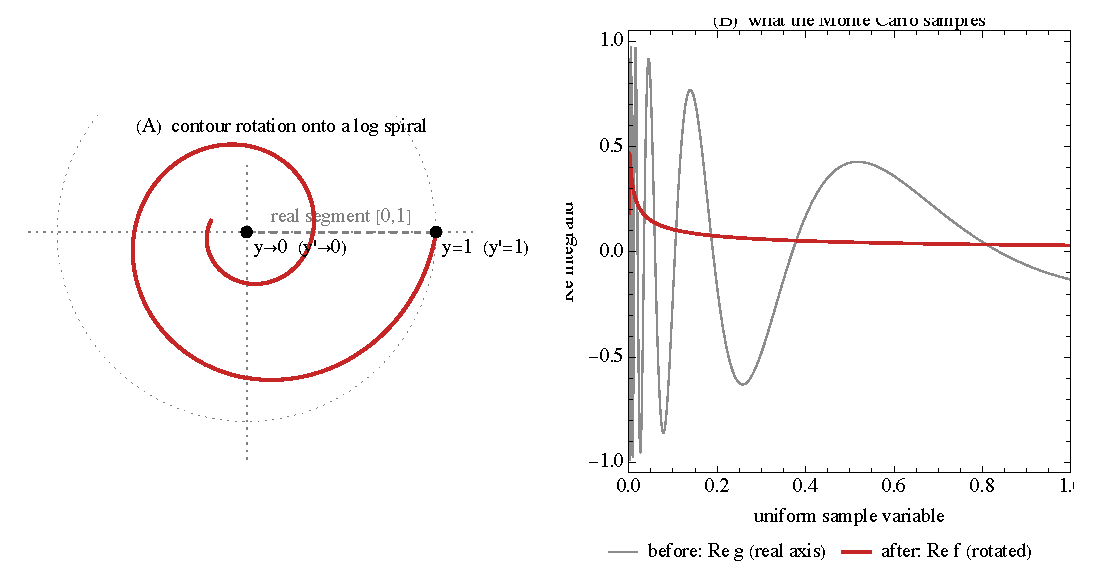
\includegraphics[width=\textwidth]{complex_flatten_spiral.pdf}
\caption{Complex flattening for sector $\rho_+$ of \eqref{eq:cx-int}
($a = 1-6i$). \textbf{(A)} The substitution $y=(y')^{1/a}$ maps the real
segment $[0,1]$ (dashed) onto a logarithmic spiral (red) running from $y=1$
into $y=0$; the dotted curve is the unit circle. \textbf{(B)} The real part of
the integrand as a function of the uniform sample variable: before the rotation
\eqref{eq:cx-g} it oscillates with diverging frequency near the origin (grey);
after the rotation \eqref{eq:cx-f} it is smooth (red). The two contours give
the \emph{same} integral, by analytic continuation.}
\label{fig:cx-spiral}
\end{figure}

\paragraph{Why this is legal, and what it buys.} The move is not an
approximation: $y=(y')^{1/a}$ is an analytic change of variables, equivalently
(Cauchy's theorem) a deformation of the real contour onto the spiral --- the
integrand $y^{a-1}(1+y)^{B}$ is holomorphic in the swept region, its only
branch points being $y=-1$ (far from the spiral, which stays in $|y|\le1$) and
the shared, integrable endpoint $y=0$ (where $\operatorname{Re}a=1>0$). It is
precisely the analytic continuation in $a$ of the real-exponent flattening
(Section~\ref{sec:complex-exponents}): for real $a>0$ the ``spiral'' is just the
real segment reparametrised; a nonzero $\operatorname{Im}a$ tilts it off the
axis. Numerically both contours return the identical sector value
$0.0619 - 0.0541\,i$, and the reassembled total matches $1/(1-6i)$ to machine
precision. The payoff is variance: over $2\times10^{5}$ uniform samples the
per-sample variance of the sampled integrand falls from
$(\operatorname{Var}\operatorname{Re},\operatorname{Var}\operatorname{Im})
\approx(0.138,\,0.148)$ on the real contour to $(0.0059,\,0.0084)$ on the
rotated one --- about a $20\times$ reduction, growing with $b$ as the
un-rotated oscillation gets faster. Lifting flattens a swing in
\emph{magnitude} (Section~\ref{sec:lift-example}); complex flattening flattens a
swing in \emph{phase}. Both turn a function that uniform sampling cannot resolve
into a flat $O(1)$ one, and both are exact.

%=============================================================================
\section{Dependencies}
%=============================================================================

\subsection{External Software}

\begin{description}
  \item[Polymake] (\url{https://polymake.org}) \\
    Polyhedral-computation tool, used \emph{only} by the fan-computation code \texttt{tropical\_fan.wl} (a black box from this manual's perspective, Section~\ref{sec:fanblackbox}). Must be installed and accessible on \texttt{PATH}, or in one of: \texttt{/opt/homebrew}, \texttt{/usr/local}, \texttt{/usr} (override via \texttt{\$TropicalFanPolymakePath}). Can be skipped entirely with \texttt{\$SkipPolymakeLoad = True} when explicit \texttt{fanData} is supplied. \textbf{Installation guide: Section~\ref{sec:polymake-install}.}

  \item[g++ (GCC C++ compiler)] ~\\
    C++17 standard required (\texttt{-std=c++17}). OpenMP support recommended (\texttt{-fopenmp}) for parallel kinematic evaluation. If OpenMP linking fails (common on macOS with clang), the code auto-retries without \texttt{-fopenmp}.

  \item[Wolfram Mathematica (version 12.0+)] ~\\
    The symbolic computation engine. Required for running all \texttt{.wl} files. \texttt{wolframscript} used for command-line execution.

  \item[CUBA (optional)] (\url{https://feynarts.de/cuba/}) \\
    Multidimensional integration library (Vegas, Suave, Divonne, Cuhre). Used \emph{only} by the independent cross-check examples in \texttt{EXAMPLES/tropical\_eval\_examples3.wl}, which integrate the original (un-decomposed) integrand directly and compare against the tropical pipeline. Install via Homebrew (\texttt{brew install cuba}) or build from source. The examples probe \texttt{/opt/homebrew}, \texttt{/usr/local}, and \texttt{/usr} for \texttt{cuba.h} + \texttt{libcuba} and skip gracefully with a message if not found.
\end{description}

\subsection{Installing Polymake}\label{sec:polymake-install}

Polymake is the only non-trivial dependency to install, and it is needed
\emph{only} to compute fans (Section~\ref{sec:fanblackbox}); if you supply
\texttt{fanData} explicitly and set \texttt{\$SkipPolymakeLoad = True}, you can
skip this section entirely. The package drives Polymake through its
command-line executable (it shells out to \texttt{polymake} with a short Perl
script that uses the \texttt{polytope} application), so a full working
\texttt{polymake} binary on disk is required --- a library-only build is not
enough.

\paragraph{macOS (recommended: Homebrew).}
\begin{lstlisting}[language=bash]
brew install polymake
\end{lstlisting}
This installs the binary at \texttt{/opt/homebrew/bin/polymake} on
Apple-silicon Macs (or \texttt{/usr/local/bin/polymake} on Intel Macs), both
of which are auto-detected (see \emph{How the package finds Polymake}, below).
The formula
pulls in the required Perl, GMP, MPFR, FLINT, PPL, and boost dependencies
automatically. The first \texttt{polymake} invocation rebuilds its internal
caches and can take a minute or two; subsequent calls are fast. This manual
was validated against \textbf{Polymake 4.15} installed this way.

\paragraph{Linux (distribution packages).}
\begin{lstlisting}[language=bash]
# Debian / Ubuntu
sudo apt-get install polymake

# Fedora
sudo dnf install polymake

# Arch (AUR)
yay -S polymake
\end{lstlisting}
These place the binary at \texttt{/usr/bin/polymake} or
\texttt{/usr/local/bin/polymake}, both auto-detected. Distribution packages
are sometimes older than the upstream release; any version in the 3.x--4.x
range exposing the \texttt{polytope} application's \texttt{VERTICES} property
works.

\paragraph{Building from source (clusters, or for the latest release).}
When no package is available --- e.g.\ on an HPC login node without root ---
build from the official tarball:
\begin{lstlisting}[language=bash]
# Prerequisites: a C++14 compiler, Perl >= 5.16, GMP, MPFR,
# libxml2, boost, ninja, and (optionally) FLINT/PPL.
wget https://polymake.org/lib/exe/fetch.php/download/polymake-4.15.tar.bz2
tar xjf polymake-4.15.tar.bz2 && cd polymake-4.15
./configure --prefix=$HOME/polymake   # pick any writable prefix
ninja -C build/Opt
ninja -C build/Opt install
\end{lstlisting}
Add the install prefix to your \texttt{PATH} (\texttt{export
PATH=\$HOME/polymake/bin:\$PATH}) or point the package straight at the binary
(see \emph{How the package finds Polymake}, below). Full upstream
instructions:
\url{https://polymake.org/doku.php/install/install}.

\paragraph{Verifying the installation.}
\begin{lstlisting}[language=bash]
polymake --version
# polymake version 4.15 ...

# Confirm the polytope application + VERTICES work end to end:
polymake "use application 'polytope';
          my $c = cube(2);
          print $c->VERTICES;"
\end{lstlisting}
The second command should print the four vertices of the unit square in
homogeneous coordinates. If both succeed, the package will drive Polymake
correctly.

\paragraph{How the package finds Polymake.}\label{sec:polymake-detect}
On load, the variable \texttt{\$TropicalFanPolymakePath} is set by probing the
following locations in order, taking the first that exists:
\begin{lstlisting}[language=bash]
/opt/homebrew/bin/polymake     # Homebrew, Apple silicon
/usr/local/bin/polymake        # Homebrew (Intel) / source default
/usr/bin/polymake              # Linux distribution packages
polymake                       # fallback: resolved via $PATH
\end{lstlisting}
For a non-standard location, set the path \emph{before} loading the package:
\begin{lstlisting}[language=Mathematica]
$TropicalFanPolymakePath = "/home/me/polymake/bin/polymake";
Get["tropical_eval.wl"];
\end{lstlisting}
A failed Polymake call raises \texttt{TropicalFan::polymake} with the
captured \texttt{stderr}; the most common causes are a binary not on the
probed paths (set \texttt{\$TropicalFanPolymakePath}) and a first-run cache
rebuild that exceeded the process timeout (re-run once warmed up).

\subsection{Internal Dependencies}

\begin{itemize}
  \item \texttt{tropical\_fan.wl} must be loaded before \texttt{tropical\_eval.wl}; the latter \texttt{Get}s it internally, unless \texttt{\$SkipPolymakeLoad} is set to \texttt{True} first.
  \item No external Wolfram packages required beyond the core installation.
\end{itemize}

%=============================================================================
\section{Usage and Workflow}
%=============================================================================

\subsection{Minimal Convergent Integral}

\begin{lstlisting}[language=Mathematica]
(* Load the package *)
Get["tropical_eval.wl"];

(* Define the integrand *)
poly = 1 + 2*x[1]^2 + x[2]^2 + x[1]*x[2]^2;
vars = {x[1], x[2]};

spec = <|
  "Polynomials"         -> {poly},
  "MonomialExponents"   -> {0, 0},
  "PolynomialExponents" -> {-2},
  "Variables"           -> vars,
  "KinematicSymbols"    -> {},
  "RegulatorSymbol"     -> None
|>;

(* Compute the fan *)
verts   = PolytopeVertices[poly^(-1), vars];
fanData = ComputeDecomposition[verts];

(* Validate against NIntegrate *)
vr = ValidateDecomposition[spec, fanData, {}, 3];
Print["Relative error: ", vr["RelativeError"]];

(* Full MC evaluation *)
results = EvaluateTropicalMC[spec, fanData, {}];
\end{lstlisting}

\subsection{Kinematic Scan (Many Evaluation Points)}

\begin{lstlisting}[language=Mathematica]
Get["tropical_eval.wl"];

(* Polynomial with kinematic-dependent coefficients *)
poly = c0 + c1*x[1]^2 + c2*x[2]^2;

spec = <|
  "Polynomials"         -> {poly},
  "MonomialExponents"   -> {0, 0},
  "PolynomialExponents" -> {-2},
  "Variables"           -> {x[1], x[2]},
  "KinematicSymbols"    -> {c0, c1, c2},
  "RegulatorSymbol"     -> None
|>;

(* Fan uses unit coefficients -- structure only *)
proxyPoly = 1 + x[1]^2 + x[2]^2;
verts = PolytopeVertices[proxyPoly^(-1), vars];
fanData = ComputeDecomposition[verts];

(* Define 7200 kinematic points *)
kinPoints = Table[{1.0, 0.5+0.01*i, 1.0+0.005*i}, {i, 7200}];

(* Evaluate: one compilation, parallel execution *)
results = EvaluateTropicalMC[spec, fanData, kinPoints];
\end{lstlisting}

\textbf{Note:} The fan decomposition depends only on the Newton polytope structure (which monomials appear), not on numerical coefficients. The same decomposition works for all kinematic points, requiring only one C++ compilation.

\subsection{Extreme Coefficients via Lifting}

\begin{lstlisting}[language=Mathematica]
Get["tropical_eval.wl"];

(* Small coefficient 10^-4: decomposition is exact, but plain
   uniform MC is heavy-tailed.  Lift the coefficient instead. *)
spec = <|
  "Polynomials"         -> {1 + 10^-4 x[1]^2 + x[2]^2 + x[1] x[2]^2},
  "MonomialExponents"   -> {0, 0},
  "PolynomialExponents" -> {-2},
  "Variables"           -> {x[1], x[2]},
  "KinematicSymbols"    -> {},
  "RegulatorSymbol"     -> None
|>;

(* Which coefficients are extreme?  SuggestedK is the auto-chosen anchor
   exponent (kStar rule, Section "Choosing the Lift Anchor z0"); here k = 2. *)
DetectExtremeCoefficients[spec, 1000]

(* Simplest path: let the kStar rule pick k (= 2 here) automatically. *)
result = EvaluateTropicalMCLifted[spec, {{}}, "LiftRules" -> Automatic,
  "NSamples" -> 10^6];

(* Equivalent explicit form -- lift 10^-4 x1^2 -> z^2 x1^2, anchor z0 = 1/100.
   Use this to override the rule, or "AnchorRule" -> "Unit" for the legacy
   k = 1, or "BandEdgeGuard" -> True for the +1 band-edge correction. *)
result = EvaluateTropicalMCLifted[spec, {{}},
  "LiftRules" -> {<|"PolyIndex" -> 1,
                    "ExponentVector" -> {2, 0}, "k" -> 2|>},
  "NSamples" -> 10^6];

result["Results"][[1]]  (* <|"Re" -> ..., "ReErr" -> ..., ...|> *)
\end{lstlisting}

See Example~20 in \texttt{EXAMPLES/tropical\_eval\_examples2.wl} for the full worked version, including the plain-vs-lifted variance comparison and the exactness check via \texttt{ValidateLiftedDecomposition}.

\subsection{Command-Line Execution}

% NOTE: run the C++/MC scripts ONE AT A TIME -- they share INTERFILES/ with
% fixed filenames (tropical_mc, tropical_mc_generated.cpp, mc_results.txt), so
% two concurrent jobs in the same working directory clobber each other.
\begin{lstlisting}[language=bash]
# Quick smoke test (Example 1 only)
wolframscript -file EXAMPLES/test_quick.wl

# C++ code generation and execution test
wolframscript -file EXAMPLES/test_cpp.wl

# Examples 1-14 (general pipeline)
wolframscript -file EXAMPLES/tropical_eval_examples.wl

# Examples 1-14 followed by the 6-test RunAllTests validation suite
wolframscript -file EXAMPLES/run_validation_suite.wl

# Examples 15-20 (complex exponents, small coefficients, lifting)
wolframscript -file EXAMPLES/tropical_eval_examples2.wl

# Examples 21-23 (independent cross-checks: exact Gamma + CUBA)
wolframscript -file EXAMPLES/tropical_eval_examples3.wl

# Examples 24-27 (lifting with complex, small-magnitude coefficients)
wolframscript -file EXAMPLES/tropical_eval_examples4.wl

# SeedBase runtime-argv override (re-run one binary under several seeds)
wolframscript -file EXAMPLES/test_seedbase.wl

# Lifted-pipeline test suite (Test 23)
wolframscript -file EXAMPLES/test_lifted.wl

# Complex-coefficient lifted test suite (Test 24)
wolframscript -file EXAMPLES/test_complex_lifted.wl

# CUBA cross-check of ALL test-suite integrals (requires CUBA)
wolframscript -file EXAMPLES/test_cuba.wl

# MC vs VEGAS parity demonstration (requires CUBA)
wolframscript -file EXAMPLES/test_vegas.wl

# Fan computation examples
wolframscript -file EXAMPLES/tropical_fan_examples.wl
\end{lstlisting}

%=============================================================================
\section{Examples Directory}
%=============================================================================

The \texttt{EXAMPLES/} directory contains worked examples and validation tests.

\subsection*{\texttt{tropical\_eval\_examples.wl} --- Examples 1--14}

\begin{center}
\begin{tabular}{cl}
\toprule
\textbf{Example} & \textbf{Description} \\
\midrule
1 & Basic 2D convergent integral \\
2 & Complex exponents ($B_j$ with imaginary part) \\
3 & Kinematic-dependent integral (coefficients are parameters) \\
4 & Tropical factoring step-by-step walkthrough \\
5 & \texttt{MmaToC} expression converter demonstration \\
6 & C++ code generation and execution (full pipeline) \\
7 & C++ with kinematic scan (multiple evaluation points) \\
8 & \texttt{ParsePolynomial} utility function \\
9 & Multiple polynomials (2 factors in denominator) \\
10 & Non-trivial numerator (1 polynomial, positive $B$) \\
11 & Non-trivial numerator (2 polynomials) \\
12 & Numerator with kinematic-dependent coefficients \\
13 & 3D convergent integral (6 rays, 8 sectors) \\
14 & 4D convergent integral (8 rays, 14 sectors) \\
\bottomrule
\end{tabular}
\end{center}

\subsection*{\texttt{tropical\_eval\_examples2.wl} --- Examples 15--20: Complex Exponents and Small Coefficients}

All six examples are convergent and cross-checked against \texttt{NIntegrate}.

\begin{center}
\begin{tabular}{cl}
\toprule
\textbf{Example} & \textbf{Description} \\
\midrule
15 & Two polynomials, both raised to complex exponents \\
   & $(1{+}x_1{+}x_2)^{-(3/2+i/2)}\,(1{+}x_1 x_2)^{-(1-i/3)}$ \\
16 & Complex monomial exponents and complex polynomial exponent \\
   & $x_1^{1/2+i/3}\, x_2^{-1/4-i/5}\, P^{-(2+i)}$ \\
17 & Full C++ MC via \texttt{EvaluateTropicalMC} with complex exponent \\
   & $P_\lambda^{-(2+i/2)}$, kinematic scan over $\lambda$, MC vs.\ \texttt{NIntegrate} \\
18 & Small coefficients ($10^{-4}$, $10^{-3}$): exactness + variance diagnostics \\
   & via \texttt{DetectExtremeCoefficients} / \texttt{CheckFlatteningMagnitude} \\
19 & Small coefficients \emph{and} complex exponent combined \\
   & $(1 + 10^{-3}x_1^2 + x_2^2 + 10^{-2}x_1 x_2^2)^{-(2+i/2)}$ \\
20 & Lifting a small coefficient ($10^{-4} \to z^2$, $z_0 = 1/100$): \\
   & exactness via \texttt{ValidateLiftedDecomposition}, then plain-vs-lifted \\
   & MC comparison (heavy tail vs.\ controlled variance); Step~7 demonstrates \\
   & the automatic anchor (\texttt{"LiftRules" -> Automatic}, the $k^{*}$ rule) \\
\bottomrule
\end{tabular}
\end{center}

\subsection*{\texttt{tropical\_eval\_examples3.wl} --- Examples 21--23: Independent Cross-Checks}

These examples validate the pipeline against methods that share no code, algorithm, or CAS with it (or with \texttt{NIntegrate}): an exact Gamma-function closed form, and the \textbf{CUBA} library integrating the \emph{original} integrand directly on $[0,\infty)^n$ via the compactification $x_i = t_i/(1-t_i)$. The generator that turns any numeric \texttt{IntegrandSpec} into a self-contained two-component (Re, Im) CUBA program lives in the shared helper file \texttt{cuba\_common.wl} (\texttt{generateCubaSource} / \texttt{runCubaCheck}); it is also used by \texttt{test\_cuba.wl}, which cross-checks every test-suite integral (Section~\ref{sec:cubacheck}). CUBA is an optional dependency (Section~8.1); the CUBA parts skip gracefully if it is not installed.

\begin{center}
\begin{tabular}{cl}
\toprule
\textbf{Example} & \textbf{Description} \\
\midrule
21 & Exact Beta/Gamma closed form, complex exponents: \\
   & $\int x_1^{a_1-1} x_2^{a_2-1} (1{+}x_1{+}x_2)^{-b} = \frac{\Gamma(a_1)\Gamma(a_2)\Gamma(b-a_1-a_2)}{\Gamma(b)}$ \\
   & ($a_1 = \tfrac54 + \tfrac{i}{3}$, $a_2 = \tfrac32 - \tfrac{i}{5}$, $b = 5 + \tfrac{i}{2}$); exact vs.\ \texttt{NIntegrate} \\
   & vs.\ tropical MC vs.\ CUBA Cuhre (agreement to $3{\times}10^{-8}$) \\
22 & Small coefficient $10^{-4}$ (Example 20's integrand): CUBA Cuhre \\
   & (deterministic) and Vegas (importance-sampling MC) vs.\ lifted \\
   & tropical MC --- three unrelated algorithms agree on $\approx 13.0901$ \\
23 & Complex exponent + small coefficients (Example 19's integrand): \\
   & CUBA Cuhre two-component reference vs.\ unlifted tropical MC \\
   & (honest but large error bars; lifting unavailable for complex $B$) \\
\bottomrule
\end{tabular}
\end{center}

\subsection*{\texttt{tropical\_eval\_examples4.wl} --- Examples 24--27: Lifting with Complex, Small-Magnitude Coefficients}\label{sec:complex-coeff-examples}

Examples~2 and 15--19 made the integrand complex through the \emph{exponents}; Example~20 lifted a small but \emph{real} coefficient. This file combines the two regimes: a polynomial coefficient that is itself \emph{complex} and of very small magnitude, fed through the lifting module. The complex coefficient is split into a real anchor $z_0 = |C|^{1/k}$ and an $\mathcal{O}(1)$ phase residual $c = C/z_0^k$ (Section~\ref{sec:lifting}, ``Complex coefficients''), so the lifted decomposition stays exact and the integral is correctly complex-valued. All four are cross-checked against direct \texttt{NIntegrate} (Example~24 additionally runs the full C++ MC, requiring g++).

\begin{center}
\begin{tabular}{cl}
\toprule
\textbf{Example} & \textbf{Description} \\
\midrule
24 & Single small complex coefficient $(1{+}i)10^{-4}$, $k=2$: detection, lift, \\
   & identity, lifted-decomposition exactness (Re \emph{and} Im), and plain-vs- \\
   & lifted C++ MC --- plain MC is wildly heavy-tailed, lifted MC tracks the \\
   & complex reference $\approx 11.63 - 2.58\,i$ in both components \\
25 & Very small $(1{+}i)10^{-7}$ with the \emph{automatic} anchor: the $k^{*}$ rule \\
   & grows the anchor exponent to $k=3$ as $|C|$ shrinks; decomposition exact \\
26 & Two small complex coefficients lifted against one anchor (multi-rule): \\
   & residual phases stay $\mathcal{O}(1)$; the round-trip is exact for both at once \\
27 & Purely imaginary coefficient $i\,10^{-4}$ (residual $= i$), plus the boundary \\
   & case: a complex \emph{exponent} $B = -(2{+}i/2)$ correctly fires \texttt{liftcomplex} \\
\bottomrule
\end{tabular}
\end{center}

\subsection*{Other Example Files}

\begin{description}
  \item[\texttt{tropical\_fan\_examples.wl}] --- Fan decomposition examples for various polytopes.
  \item[\texttt{test\_quick.wl}] --- Minimal test running only Example~1.
  \item[\texttt{test\_cpp.wl}] --- Tests C++ code generation, compilation, and execution.
  \item[\texttt{run\_validation\_suite.wl}] --- Runs Examples~1--14 (by loading \texttt{tropical\_eval\_examples.wl}) and then invokes \texttt{RunAllTests[]}, the 6-test validation suite (Section~\ref{sec:sixtest}). The examples file \emph{defines} \texttt{RunAllTests[]} but never calls it, so this runner is the way to exercise the suite from the command line; it exits non-zero if any test fails.
  \item[\texttt{test\_seedbase.wl}] --- Tests the \texttt{SeedBase} runtime-argv override: compiles one binary, then re-runs it under several seeds, asserting determinism (same seed $\Rightarrow$ identical output), that omitting \texttt{argv[5]} equals passing the compile-time default, distinct MC streams across seeds, and each stream within $5\sigma$ of $\pi/8$.
  \item[\texttt{test\_lifted.wl}] --- Test 23: the lifted-integral pipeline (four subtests, see Section~\ref{sec:test23}).
  \item[\texttt{test\_complex\_lifted.wl}] --- Test 24: lifting with \emph{complex}, small-magnitude coefficients (four subtests, see Section~\ref{sec:test24}). The automated PASS/FAIL companion to Examples~24--27; exits non-zero on any failure.
  \item[\texttt{cuba\_common.wl}] --- Shared CUBA cross-check generator (used by \texttt{tropical\_eval\_examples3.wl} and \texttt{test\_cuba.wl}).
  \item[\texttt{test\_cuba.wl}] --- CUBA cross-check of all test-suite integrals (Section~\ref{sec:cubacheck}).
  \item[\texttt{test\_vegas.wl}] --- MC vs.\ VEGAS parity demonstration: runs each spec through the pipeline with \texttt{Integrator -> "MC"} and \texttt{"VEGAS"} and asserts they return the same value within combined error, with VEGAS 1--3 orders tighter (Section~\ref{sec:vegas}; requires CUBA).
  \item[\texttt{prompt\_tropical\_mc.txt}] --- Original development specification.
\end{description}

%=============================================================================
\section{Validation and Testing}
%=============================================================================

\subsection{6-Test Suite (\texttt{RunAllTests[]})}\label{sec:sixtest}

\texttt{RunAllTests[]} is \emph{defined} in \texttt{tropical\_eval\_examples.wl} but not called there; run it from the command line via \texttt{wolframscript -file EXAMPLES/run\_validation\_suite.wl}, which first executes Examples~1--14 and then invokes the suite (exiting non-zero on any failure). The v2 suite covers convergent integrals only (the divergent and IBP tests, formerly Tests 3--4 and 8--22, were removed along with the divergence machinery):

\begin{description}
  \item[Test 1:] Convergent 2D, real exponents ($A = 2, 3$). Sector sum vs.\ direct \texttt{NIntegrate}.
  \item[Test 2:] Convergent 2D, complex exponent ($A = 2 + 0.5i$). Tests log-exp evaluation with a complex-valued integrand.
  \item[Test 3v2:] Negative tests. Part~A: an $\varepsilon$-regulated spec must fail with \texttt{noregulator}. Part~B: a regulator-free but divergent spec must fail with \texttt{divergentinput}.
  \item[Test 5:] 100-point kinematic scan with complex exponent; sector decomposition verified at 5 representative points.
  \item[Test 6:] Large coefficient range ($10^{-4}$ to $10^8$, three cases). The tropically dominant monomial need not be the numerically largest one; the factoring is exact regardless.
  \item[Test 7:] 3D and 4D integrals. 3D: 6 rays, 8 sectors; 4D: 8 rays, 14 sectors.
\end{description}

\subsection{Test 23: Lifted Pipeline (\texttt{test\_lifted.wl})}\label{sec:test23}

\begin{description}
  \item[23A (exactness):] Toy~1, $P = 1 + x_1 + 10^{-6} x_2$, $B = -3$, exact value $500000$. Uses an explicit fan (the lifted polytope is degenerate). PASS: relative error $< 0.5\%$ and exactly 3 \texttt{EmptyDomain} sectors dropped.
  \item[23B (end-to-end C++):] $P = 1 + 10^6 x_1^2 + x_2^2 + x_1 x_2^2$, $B = -2$, lifted with $k = 2$ via \texttt{EvaluateTropicalMCLifted}. PASS: within 1\% of \texttt{NIntegrate} and within $4\sigma$ of the MC error bar.
  \item[23C (error paths):] (i) complex polynomial exponent must fire \texttt{liftcomplex}; (ii) a handcrafted sector where every pivot yields a non-positive $\tilde{a}$ component must fire \texttt{liftnopivot}.
  \item[23D (EmptyDomain drops):] Toy~0, $P = 1 + 10^6 x_1$, $B = -2$, $k = 1$ ($z_0 = 10^6$). PASS: dropped sectors $> 0$ and relative error $< 0.1\%$.
\end{description}

\subsection{Test 24: Lifting with Complex, Small-Magnitude Coefficients (\texttt{test\_complex\_lifted.wl})}\label{sec:test24}

The automated PASS/FAIL companion to Examples~24--27 (Section~\ref{sec:complex-coeff-examples}), confirming that the auxiliary-variable module is correct when a polynomial carries a \emph{complex} coefficient of very small magnitude. The script exits non-zero on any failure.

\begin{description}
  \item[24A (single complex coeff, full C++):] $P = 1 + (1{+}i)10^{-4} x_1^2 + x_2^2 + x_1 x_2^2$, $B = -2$, $k = 2$. PASS gates: \texttt{DetectExtremeCoefficients} flags $|C| = \sqrt{2}\,10^{-4}$ with $k^{*} = 2$; the lift identity holds and the residual has unit modulus; \texttt{ValidateLiftedDecomposition} is exact ($\sim$$10^{-5}$) in both Re and Im; the C++ MC lands within $5\sigma$ in both components; and the generated source emits a \texttt{cx(...)} literal with no broken \texttt{CForm} token.
  \item[24B (very small, automatic $k^{*}$):] $(1{+}i)10^{-7}$; the \texttt{kStar} rule returns $k = 3$ and the lifted decomposition is exact ($\sim$$10^{-7}$).
  \item[24C (multi-rule):] two small complex coefficients $(1{+}i)10^{-4}$ and $(1{-}2i)10^{-4}$ lifted against one anchor; residual magnitudes stay $\mathcal{O}(1)$, the round-trip identity holds, and the decomposition is exact ($\sim$$10^{-6}$).
  \item[24D (boundary):] a complex polynomial \emph{exponent} $B = -(2{+}i/2)$ (real coefficient) must still fire \texttt{liftcomplex} --- complex coefficients are liftable, complex exponents are not.
\end{description}

Measured at the time of writing: all four parts PASS. Sector sums agree with direct \texttt{NIntegrate} of the complex integrand to $6\times10^{-7}$--$7\times10^{-6}$; the C++ lifted MC for 24A reproduces $11.63 - 2.58\,i$ within its error bars in both components.

\subsection{Independent Cross-Checks: Exact Closed Form and CUBA (Examples 21--23)}\label{sec:cubacheck}

Beyond the \texttt{NIntegrate}-based validation used throughout, \texttt{tropical\_eval\_examples3.wl} (in \texttt{EXAMPLES/}) checks the pipeline against fully independent references (measured values at the time of writing):

\begin{itemize}
  \item \textbf{Exact Gamma closed form} (Example 21): the generalized Beta integral with complex exponents $a_1 = 5/4 + i/3$, $a_2 = 3/2 - i/5$, $b = 5 + i/2$. Agreement: CUBA Cuhre $3{\times}10^{-8}$ relative; \texttt{NIntegrate} $2{\times}10^{-6}$; tropical sector sum $9{\times}10^{-6}$; tropical MC within its $\sim 10^{-4}$ error bars.
  \item \textbf{CUBA Cuhre} (deterministic globally adaptive cubature) on the direct, compactified integrand: reproduces the small-coefficient reference $13.09008897$ and the complex value $18.4048601 - 8.4410360\,i$ to $10^{-7}$--$10^{-8}$, confirming \texttt{NIntegrate} independently.
  \item \textbf{CUBA Vegas} (adaptive importance-sampling MC): an unrelated Monte Carlo that converges on the heavy-tailed small-coefficient integrand where plain uniform sampling fails, agreeing within $1\sigma$.
\end{itemize}

\paragraph{Suite-wide CUBA cross-check (\texttt{test\_cuba.wl}).} The script \texttt{EXAMPLES/test\_cuba.wl} integrates \emph{every} convergent integral of the validation suite with CUBA Cuhre applied directly to the original integrand --- Test~1 ($A = 2, 3$), Test~2 (complex exponent), Test~5 (five representative kinematic points), Test~6 (Cases A/B/C, plus a lifted-MC re-check of Case~A, which equals Test~23B's integral), Test~7 (3D and 4D), and the lifted-test integrals 23A and 23D (with their exact values $5{\times}10^5$ and $10^{-6}$) --- and gates the tropical sector sum (1\%; 2\% for 4D, 5\% for the PG2 case 6C) and the tropical MC ($5\sigma$) against it. Test~6B's plain MC is reported without a gate (heavy tail from the $10^{-4}$ constant term, cf.\ Example~20). Test~3v2 contains only negative tests (nothing to integrate).

Measured at the time of writing: \textbf{all 16 cases pass}. Sector sums agree with Cuhre to $4{\times}10^{-6}$--$4{\times}10^{-4}$ ($1.3{\times}10^{-3}$ for the PG2 case 6C); gated MCs land at $0.05$--$1.9\sigma$. Cuhre also pins down reference values for the extreme-coefficient cases (Test 6A $= 7.850075{\times}10^{-4}$, 6B $= 144.0578$, 6C $= 1.684581{\times}10^{-3}$) and resolves both lifted-test geometries --- Test 23A's boundary sliver ($5{\times}10^5$ to $2{\times}10^{-8}$ relative) and Test 23D's $10^{-6}$-wide peak ($10^{-6}$ to $10^{-10}$).

The \texttt{CC/} directory contains cross-validation of the \emph{original} package against \textbf{FIESTA}, an independent sector decomposition code used in the physics community: a $\pi/8$ convergent integral (agreement to 6 decimal places), a divergent Gamma-function integral (pole matches exactly), and a full 5D cosmological integral (bubblepp presector~1; results match FIESTA within $2\sigma$ of the MC error, with $1/\sqrt{N}$ error scaling verified from $N = 5\times10^4$ to $10^7$).

These results predate v2. Scripts in \texttt{CC/} that call the removed divergent/IBP functions (\texttt{IdentifyDivergences}, \texttt{ProcessDivergentSector}, \texttt{EvaluateTropicalMCIBP}, \ldots) are retained as historical artifacts and are \emph{not} runnable against v2.

%=============================================================================
\section{Limitations and Caveats}
%=============================================================================

\begin{enumerate}
  \item \textbf{Convergent integrals only.} v2 rejects $\varepsilon$-regulated specifications (\texttt{noregulator}) and divergent sectors (\texttt{divergentinput}). For pole extraction use the original \texttt{TROPICAL\_MONTE\_CARLO} package.

  \item \textbf{Polynomial coefficients.} The default and best-conditioned case is real positive coefficients, for which $\log(P_j)$ is real-valued and the cleared $Q_k \geq c_{\mathrm{dom}} > 0$ estimate of Section~\ref{sec:alg-factoring} holds exactly. \emph{Complex} coefficients are also supported --- both directly (the C++ pipeline carries all polynomial values as \texttt{std::complex<double>}) and through the lifting module, which splits a small complex coefficient into a real anchor $z_0 = |C|^{1/k}$ and an $\mathcal{O}(1)$ phase residual (Sections~\ref{sec:lifting},~\ref{sec:complex-coeff-examples}). The one proviso is the branch of $\log Q_k$: results use the principal branch, which is the correct, \texttt{NIntegrate}-consistent value provided no $Q_k$ winds around $0$ on $[0,1]^n$ (guaranteed when the dominant constant term keeps $Q_k$ near the positive real axis, as for a small complex perturbation of a positive polynomial). Genuinely complex integrands otherwise arise only from the exponents $A_i$ and $B_j$.

  \item \textbf{Monte Carlo convergence and heavy tails.} Accuracy scales as $1/\sqrt{N}$. When coefficients span many orders of magnitude, some sectors become heavy-tailed: the MC estimate \emph{and its sample error bar} can both be too small at moderate $N$ (the rare high-magnitude region is never sampled; see Example~20). Use \texttt{CheckFlatteningMagnitude} to locate such sectors and the lifting module to mitigate them.

  \item \textbf{Lifting restrictions.} Lifting requires real polynomial exponents $B_j$ (\texttt{liftcomplex} otherwise). When the lifted polynomial has too few monomials, its Newton polytope is lower-dimensional and the automatic fan fails (\texttt{liftdegenerate}); supply an explicit \texttt{"FanData"}. Lifted sectors with \texttt{HasConstantTerm -> False} may have infinite true variance, making sample error bars unreliable (see \texttt{SUMMARY.txt} \S8f). \texttt{DetectExtremeCoefficients} skips symbolic (kinematic) coefficients, whose magnitude is unknown at lift time.

  \item \textbf{Polymake dependency.} External tool, not bundled; required only for computing fans (\texttt{tropical\_fan.wl}). With \texttt{\$SkipPolymakeLoad = True} and explicit \texttt{fanData}, the evaluation pipeline runs without it.

  \item \textbf{Newton polytope stability.} If kinematic parameters can cause coefficients to vanish, the Newton polytope changes and the fan must be recomputed. The code assumes fixed polytope structure across all kinematic points.

  \item \textbf{C++ compiler requirements.} \texttt{g++} with C++17 required. OpenMP optional but recommended. macOS clang may require fallback to single-threaded mode.

  \item \textbf{Double precision.} All C++ computation uses 64-bit doubles. Higher precision would require additional libraries.

  \item \textbf{Memory scaling.} Results scale linearly with the number of kinematic points. Very large scans ($\gg 10{,}000$ points) may require attention to memory.
\end{enumerate}

%=============================================================================
\section{Mathematical Properties and Why It Works}
%=============================================================================

\paragraph{Why tropical decomposition works.}
As $\mathbf{x} \to 0$ in a direction $\mathbf{w}$, the polynomial $P(\mathbf{x})$ is dominated by the monomial whose exponent vector minimizes the dot product with $\mathbf{w}$. The tropical fan exactly partitions $\mathbb{R}^n$ into regions where each monomial dominates. Within each sector, the dominant monomial is factored out, leaving a polynomial $Q(\mathbf{y})$ bounded away from zero.

\paragraph{Why flattening is important.}
Without flattening, the integrand contains factors $y_i^{a_i - 1}$ which can be highly peaked near $y_i = 0$ when $a_i$ is small. Uniform MC sampling wastes most samples away from the peak, leading to enormous variance. Flattening absorbs the $y^{a-1}$ singularity into the integration measure, converting the integrand to $\mathcal{O}(1)$ and dramatically reducing MC variance.

\paragraph{Why log-exp evaluation is stable.}
For $y \in (0, 1]$, $\log(y)$ varies smoothly in $(-\infty, 0]$. The exponential $\exp(\alpha \log y) = y^\alpha$ handles fractional and complex $\alpha$ without branch cuts or sign ambiguities. As $y \to 0^+$, the function decays or grows depending on $\mathrm{Re}(\alpha)$, but always smoothly.

\paragraph{Why tropical factoring is exact.}
The identity $P(\mathbf{y}) = \mathbf{y}^d \cdot Q(\mathbf{y})$ is algebraic, not a numerical approximation. Every monomial in $Q$ has non-negative exponents by construction. The constant term in $Q$ ensures $Q \geq \text{const} > 0$ on $[0,1]^n$. No numerical error is introduced.

\paragraph{Why lifting is exact.}
Replacing $C\,\mathbf{x}^\alpha \to z^k\,\mathbf{x}^\alpha$ and inserting $\int dz\,\delta(z - z_0)$ with $z_0 = |C|^{1/k}$ changes nothing: evaluating the lifted polynomial at $z = z_0$ reproduces the original polynomial identically (the round-trip is checked symbolically by \texttt{LiftCoefficients}; residual coefficients $c_i = C_i/z_0^{k_i}$ preserve exactness when several monomials are lifted against one anchor). The delta constraint is then resolved \emph{analytically} per sector --- the pivot substitution is a monomial change of variables, not an approximation --- so the lifted sector sum equals the original integral exactly. Sectors whose delta root lies outside the unit cube genuinely contribute zero (\texttt{EmptyDomain}). What lifting changes is only the \emph{geometry} of the decomposition: the extreme coefficient becomes part of the Newton polytope of the lifted polynomial, so the fan adapts to it and the per-sector integrands are closer to $\mathcal{O}(1)$, reducing MC variance.

\end{document}
